\documentclass{article}
    % General document formatting
    \usepackage[margin=0.7in]{geometry}
    \usepackage[parfill]{parskip}
    \usepackage[utf8]{inputenc}
    
    % Related to math
    \usepackage{amsmath,amssymb,amsfonts,amsthm}
\usepackage{graphicx}
%\usepackage{subfig}
%\usepackage{subfigure}
\usepackage{caption}
\usepackage{subcaption}
\usepackage{listings}
\usepackage[percent]{overpic}
\usepackage{xcolor,varwidth}
\usepackage{braket}

\usepackage{titling}
%\usepackage{lipsum}

\usepackage{titlesec}

\titleformat*{\section}{\Large\bfseries}
\titleformat*{\subsection}{\large\bfseries}
%\titleformat*{\subsubsection}{\large\bfseries}
%\titleformat*{\paragraph}{\large\bfseries}
%\titleformat*{\subparagraph}{\large\bfseries}
\titlespacing\section{0pt}{12pt plus 4pt minus 2pt}{0pt plus 2pt minus 2pt}
\titlespacing\subsection{0pt}{12pt plus 4pt minus 2pt}{0pt plus 2pt minus 2pt}
\titlespacing\subsubsection{0pt}{12pt plus 4pt minus 2pt}{0pt plus 2pt minus 2pt}

\pretitle{\begin{center}\large\bfseries}
\posttitle{\par\end{center}\vskip 0.01em}
\preauthor{\begin{center}\Large\ttfamily}
\postauthor{\end{center}}
\predate{\par\normalsize\centering}
\postdate{\par}


\begin{document}


\begin{center}
\textbf{\LARGE{\centering{Population Genetic Analyses of Genomic Data 2}}}\\
\textit{USN: 303039534}\\
\end{center}

%\normalsize{   }
%~\\

\section{Exercises}




\subsection{Phylogenetics}

A python script was written to construct a tree graph from the data structure provided, storing the length of each edge and the label of each node. The script also includes a topological sort function that will sort the nodes non-uniquely such that for no pair of nodes a and b with indices i and j where $i < j$ will b be a parent of a. Using this function, we include in our parsing function a subroutine that counts for each node $a$ how many total descendants it has and how many of these are leafnodes and internal nodes respectively. Finally, each node is also annotated with its total length from the rootnode.

These numbers are given in table \ref{tab:treesum} sorted from fewest to most total descendants. This also identifies node 5 as the root node and nodes 8,14,15,2,11,6,13 as leafnodes.

\begin{table}[h]
\centering
\begin{tabular}{ |c|c|c|c|c|}
\hline
 node & cumulative daughter nodes & internal nodes & leafnodes & distance from root \\
\hline
8 & 0 & 0 & 0 & 8.2 \\
14 & 0 & 0 & 0 & 8.2 \\
15 & 0 & 0 & 0 & 8.2 \\
2 & 0 & 0 & 0 & 8.2 \\
11 & 0 & 0 & 0 & 8.2 \\
6 & 0 & 0 & 0 & 8.2 \\
13 & 0 & 0 & 0 & 8.2 \\
\hline
12 & 2 & 2 & 0 & 5.5 \\
4 & 2 & 2 & 0 & 7.1 \\
7 & 2 & 2 & 0 & 3.5 \\
3 & 4 & 3 & 1 & 3.7 \\
10 & 4 & 3 & 1 & 5.2 \\
1 & 10 & 6 & 4 & 2.2 \\
5 & 14 & 8 & 6 & 0 \\
\hline
\end{tabular}
\caption{}
\label{tab:treesum}
\end{table}

b)
We include in the final column of table \ref{tab:treesum} the distance of each node from the rootnode. This shows that the length to every leafnode from the root is 8.2 units. The tree is thus consistent with an evolutionary tree where branches represent time since all current individuals (leafnodes) are equidistant from their combined most recent common ancestor (the rootnode).

We can also show this visually by plotting the tree such that the length along the y-axis corresponds to the length L between two nodes. We label each node with its node label and give the result in figure \ref{fig:tree}

\begin{figure}[h]
	\centering
	\begin{subfigure}[t]{0.55\linewidth}
		\centering
		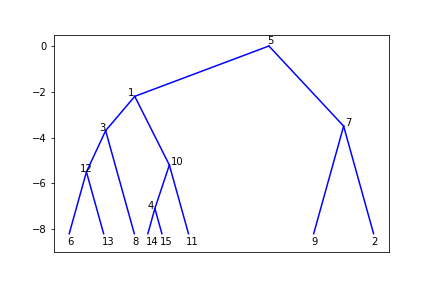
\includegraphics[width = 1.0\linewidth, trim={50 35 30 30}, clip=true]{figures/tree.png}
	\end{subfigure}
\caption{Visual representation of the tree provided in the assignment. The y axis is proportional to the branch length between nodes.}
\label{fig:tree}
\end{figure}

\newpage

c)

Given our topological sort function, we can now easily print out a relabelled tree where every daughter node has a lower number than its parent, simply by labelling each node according to its position in the reverse of the topologically sorted list.


\begin{table}[h]
\centering
\begin{tabular}{ |c|c|c|c|c|c|}
\hline
 new label & original label & cumulative daughter nodes & internal nodes & leafnodes & distance from root \\
\hline
11 & 8 & 0 & 0 & 0 & 8.2 \\
9 & 14 & 0 & 0 & 0 & 8.2 \\
8 & 15 & 0 & 0 & 0 & 8.2 \\
5 & 9 & 0 & 0 & 0 & 8.2 \\
4 & 2 & 0 & 0 & 0 & 8.2 \\
3 & 11 & 0 & 0 & 0 & 8.2 \\
2 & 6 & 0 & 0 & 0 & 8.2 \\
1 & 13 & 0 & 0 & 0 & 8.2 \\
\hline
7 & 12 & 2 & 2 & 0 & 5.5 \\
10 & 4 & 2 & 2 & 0 & 7.1 \\
6 & 7 & 2 & 2 & 0 & 3.5 \\
12 & 3 & 4 & 3 & 1 & 3.7 \\
13 & 10 & 4 & 3 & 1 & 5.2 \\
14 & 1 & 10 & 6 & 4 & 2.2 \\
15 & 5 & 14 & 8 & 6 & 0 \\
\hline
\end{tabular}
\caption{}
\label{tab:treesum2}
\end{table}

Or in the format provided in the assignment:

\begin{table}[h]
\centering
\begin{tabular}{ |c c c c c|}
\hline
14  &  12 &   1.5 &  13  &  3.0 \\  
12  &  7   &  1.8  & 11  &  4.5  \\
10  &  9   &  1.1  & 8   &  1.1  \\
15  &  14  &  2.2  & 6   &  3.5  \\
6   &  5  &   4.7 &  4   &  4.7  \\
13  &  10  &  1.9  & 3   &  3.0  \\
7   &  2   &  2.7 &  1  &   2.7 \\
\hline
\end{tabular}
\caption{}
\label{tab:treesum3}
\end{table}

\newpage


We can also use this list to plot a relabelled graph from which it is clear that the new labelling satisfies the condition that every daughter node has a lower number than its parent.

\begin{figure}[h]
	\centering
	\begin{subfigure}[t]{0.63\linewidth}
		\centering
		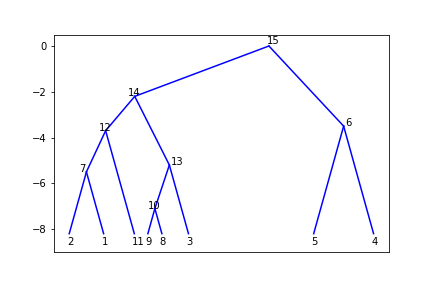
\includegraphics[width = 1.0\linewidth, trim={50 35 30 30}, clip=true]{figures/tree_relabelled.png}
	\end{subfigure}
\caption{}
\label{fig:tree_relab}
\end{figure}

\newpage










\subsection{Time-dependent selection}

We consider an organisms with 1000 polymorphic genes, each of which can be fixed in state 0 or 1. We let $f_i^a$ denote the fitness advantage of gene $i$ in state $a$ and draw it from an exponential distribution with rate parameter 100, $ f \sim \text{Exp}(\lambda = 100)$.
We assume state 1 to be beneficial and let $f_i^0 = -f_i^1$, $f_i^1 > 0$. It is assumed that no more than one gene is polymorphic at any time. Given a mutation in a gene, the probability of fixation is given by
\begin{equation}\label{eq:pfix}
p_{fix}(f_i^a) = \dfrac{1- e^{-2 f_i^a}}{1- e^{-2 N f_i^a}}
\end{equation}
Where N is the population size. The lifespan of each polymorphism is assumed to follow equation \ref{eq:lifetime} with N=100 and using the natural logarithm.
\begin{equation}\label{eq:lifetime}
\min{(10, \dfrac{2 \log{(N-1)}}{919 | f_i^a |})}
\end{equation}

We note that this particular system can be implemented in two different ways.
\begin{enumerate}
\item
In the first implementation (scenario 1), we consider consecutive mutations between the 0 and 1 states of a gene to be independent such that whenever a mutation occurs in a gene in state 1, we draw a new fitness $f_i^0 = -|f_i|$ and whenever a mutation occurs in state 0, we draw a new fitness $f_i^1 = +|f_i|$.
\item
In the other implementation (scenario 2), the relative fitnesses of states 0 and 1 are fixed and we draw all $f_i^1$ at the beginning of the simulation corresponding to the system switching between two pre-defined alleles over the course of the simulation. On one hand, this justifies always having $f_i^0 < 0$ and $f_i^1 > 0$, but on the other hand it is unlikely that a second mutation in gene $i$ will exactly reverse the effect of the first mutation. In the following, we consider both of these interpretations.
\end{enumerate}

\textit{EDIT: I answered this question prior to the clarification specifying that we are expected to consider only the second implementation. I have therefore retained a comparative analysis rather than rewriting my answer to the question.}

We simulate these two systems for 3,000,000 timesteps and plot the number of loci in state 1 for both of the two approaches in figures \ref{fig:resample_trajec} and \ref{fig:constant_trajec}. We see that in both cases, an equilibrium state of $n_1 \approx 800$ is reached after 500,000 timesteps. While the present simulations were initiated with $n_1 = 1000$, the same equilibrium state is reached from different initial conditions.

b)

We start sampling the $f$ values that lead to successful fixation after t=500,000 and run the simulation for an additional 2,500,000 timesteps. We then plot histograms showing the frequency of fixation for a given value of $f$ in figures \ref{fig:resample_hist} and \ref{fig:constant_hist} for scenario 1 and 2 as described above.

\begin{figure}[h]
	\centering
	\begin{subfigure}[t]{0.40\linewidth}
		\centering
		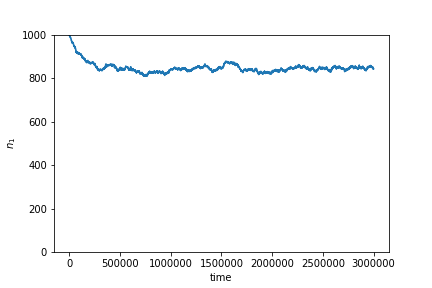
\includegraphics[width = 1.0\linewidth, trim={5 5 40 30}, clip=true]{figures/resample_selection_trajec.png}
		\subcaption{$n1$ as a function of simulated time}
		\label{fig:resample_trajec}	
	\end{subfigure}
	\hspace{0.1\linewidth}
	\begin{subfigure}[t]{0.40\linewidth}
		\centering
		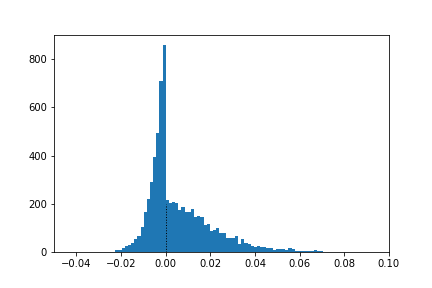
\includegraphics[width = 1.0\linewidth, trim={5 5 40 30}, clip=true]{figures/resample_selection_hist2.png}
		\caption{Frequency of fitnesses $f$ that fix in the population}
		\label{fig:resample_hist}
	\end{subfigure}
\caption{Simulation results when drawing a new $f_i$ whenever a mutation occurs (scenario 1).}
\label{fig:resample}
\end{figure}

We can explain the shape of the distribution of frequencies of fixation in the case of resampling by combining three separate distributions (figure \ref{fig:alldists}). These are\\
1. The number of alleles in states 0 and 1 respectively, since a 0 $\rightarrow$ 1 transition is associated with $f > 0$ and vice versa.\\
2. The probability with which we draw a given value of $|f|$. This is given by the exponential distribution $e^{-\lambda|f|}$ with $\lambda = 100$.\\
3. The probability with which a mutation fixates which is given by equation \ref{eq:pfix}.\\
If we multiply these three probability distributions, we arrive at a theoretical distribution that resembles the simulated data very closely (figure \ref{fig:comb}), suggesting that this is a good explanation for the observed data. The frequency distribution is thus given by
\begin{equation}\label{eq:dist1}
y \propto n_1 * exp(-|f|) * \dfrac{1- e^{-2 f}}{1- e^{-2 N f}} \,\,\,\,\, if \,\,\,\,\,\,  f < 0
\end{equation}
\begin{equation}\label{eq:dist2}
y \propto n_0 * exp(-|f|) * \dfrac{1- e^{-2 f}}{1- e^{-2 N f}}  \,\,\,\,\, if \,\,\,\,\,\, f > 0
\end{equation}

\begin{figure}[h]
	\centering
	\begin{subfigure}[t]{0.40\linewidth}
		\centering
		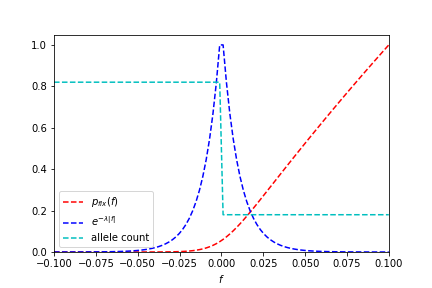
\includegraphics[width = 1.0\linewidth, trim={5 5 40 30}, clip=true]{figures/selection_dists.png}
		\subcaption{Distributions of alleles (cyan), frequency of drawing a given fitness (blue), and probability of fixation (red) as a function of fitness $f$.}
		\label{fig:alldists}	
	\end{subfigure}
	\hspace{0.1\linewidth}
	\begin{subfigure}[t]{0.40\linewidth}
		\centering
		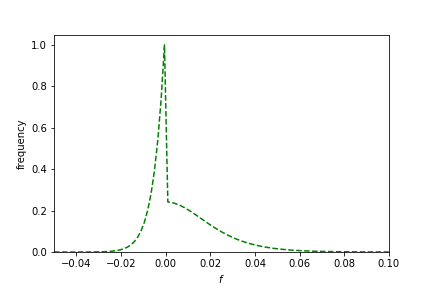
\includegraphics[width = 1.0\linewidth, trim={5 5 40 30}, clip=true]{figures/all_combined_dists.png}
		\caption{Product of the three distributions in (a). This distribution explains the observed form of the simulated data (figure \ref{fig:resample_hist}).}
		\label{fig:comb}
	\end{subfigure}
\caption{}
\label{fig:theory_resample}
\end{figure}

If instead we fix the values of $f$ at the beginning of the simulation (scenario 2), consecutive mutations are no longer independent and we instead observe a symmetric distribution of frequencies of fixation (figure \ref{fig:constant_hist}). We can understand this by considering what happens at a single site $i$. Whenever this site is in state 1, the probability of fixation is $p_1 = p_{fix}(f_0^i)$ and whenever it is in state 0 the probability of fixation is $p_0 = p_{fix}(f_1^i)$. This probability can be interpreted as a frequency of switching, and the average time of switching is thus the inverse of this frequency. However, because the state must switch back from 1 to 0 to switch from 0 to 1, in the limit of $t \rightarrow \infty$ where many switches occur, the average switching time for site i is given by the mean switching time from $0 \rightarrow 1$ and $1 \rightarrow 0$. Denoting this mean switching time $\tau_i$,
\begin{equation}
\tau_i \propto \dfrac{1}{2p_1} + \dfrac{1}{2p_0} = \dfrac{1- e^{-2 N f_i^0}}{2- 2e^{-2 f_i^0}} + \dfrac{1- e^{-2 f_i^1}}{2- 2e^{-2 N f_i^1}}
\end{equation}
The average frequency of switching for site i is thus $\omega \propto \dfrac{1}{\tau_i}$.
Since the distribution of fitnesses is given by $e^{-\lambda |f_i|}$, the probability distribution of fixation as a function of $f$ is therefore given by $\dfrac{1}{\tau_i} e^{-\lambda |f_i|} $.
This has been plotted in figure \ref{fig:simconst} and we see that it fits very well with the simulated data.

\begin{figure}[h]
	\centering
	\begin{subfigure}[t]{0.305\linewidth}
		\centering
		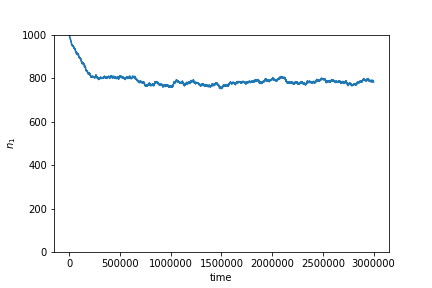
\includegraphics[width = 1.0\linewidth, trim={5 5 40 30}, clip=true]{figures/constant_selection_trajec.png}
		\subcaption{$n_1$ as a function of simulated time}
		\label{fig:constant_trajec}	
	\end{subfigure}
	\hspace{0.03\linewidth}
	\begin{subfigure}[t]{0.305\linewidth}
		\centering
		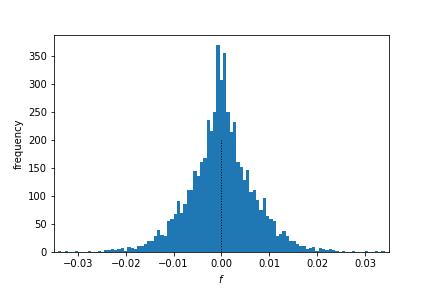
\includegraphics[width = 1.0\linewidth, trim={5 5 40 30}, clip=true]{figures/constant_selection_hist2.png}
		\caption{Frequency of fitnesses $f$ that fix in the population}
		\label{fig:constant_hist}
	\end{subfigure}
	\hspace{0.03\linewidth}
	\begin{subfigure}[t]{0.305\linewidth}
		\centering
		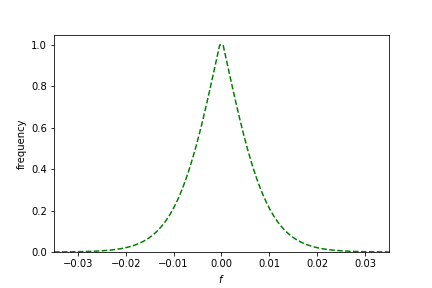
\includegraphics[width = 1.0\linewidth, trim={5 5 40 30}, clip=true]{figures/sym_combined_dists.png}
		\subcaption{Predicted frequencies of fixation given by $\dfrac{e^{-\lambda |f_i|}}{\tau_i} $}.
		\label{fig:simconst}	
	\end{subfigure}
\caption{Simulation result when $f_i$ are fixed at the beginning of the simulation (scenario 2).}
\label{fig:const}
\end{figure}

\newpage


c)

We now let the environment change at a frequency determined by a poisson distribution with rate $\tau = 5*10^{-6}$. Upon a change in environment, fitnesses of alleles 1 and 0 reverse such that $f_i^1 < 0$ and $f_i^0 > 0$ for all i. We see in figures \ref{fig:changing_resample_trajec} and \ref{fig:changing_constant_trajec} that this leads to oscillations in $n_1$ as allele 1 becomes alternatingly more and less fit compared to allele 0 at each site.

In the limit of $t \rightarrow \infty$ this averages the populations of state 0 and state 1 and leads to the resampling and fixed fitness strategies having equivalent mean behavior since consecutive fixations can now occur with the same change in fitness $\Delta f$ for a single site i in the fixed fitness model. This is illustrated in figures \ref{fig:changing_resample} and \ref{fig:changing_constant}, where we also note that we still sample fitness space less thoroughly with fixed fitnesses.

\begin{figure}[h]
	\centering
	\begin{subfigure}[t]{0.305\linewidth}
		\centering
		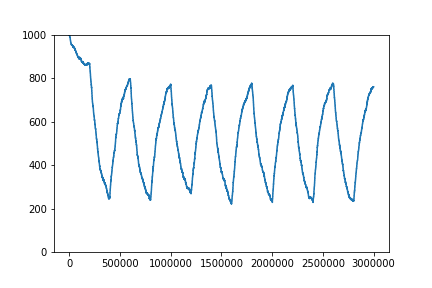
\includegraphics[width = 1.0\linewidth, trim={5 5 40 30}, clip=true]{figures/changing_resample_selection_trajec.png}
		\subcaption{$n_1$ as a function of simulated time}
		\label{fig:changing_resample_trajec}	
	\end{subfigure}
	\hspace{0.03\linewidth}
	\begin{subfigure}[t]{0.305\linewidth}
		\centering
		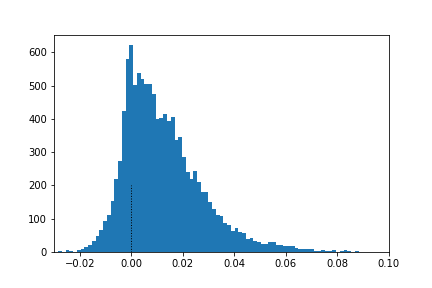
\includegraphics[width = 1.0\linewidth, trim={5 5 40 30}, clip=true]{figures/changing_resample_selection_hist2.png}
		\caption{Frequency of fitnesses $f$ that fix in the population}
		\label{fig:changing_resample_hist}
	\end{subfigure}
	\hspace{0.03\linewidth}
	\begin{subfigure}[t]{0.305\linewidth}
		\centering
		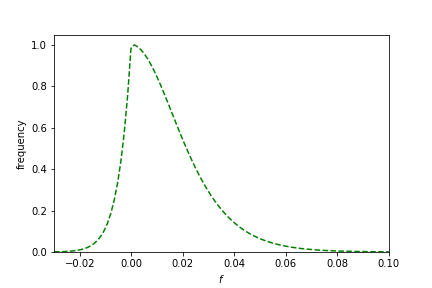
\includegraphics[width = 1.0\linewidth, trim={5 5 40 30}, clip=true]{figures/no_n_combined_dists.png}
		\caption{Predicted frequencies of fixation given by $e^{-\lambda |f|} p_{fix}(f)$}
		\label{fig:changing_resample_predict}
	\end{subfigure}
\caption{Simulated and predicted behavior of a system with resampling and changing environment (scenario 1).}
\label{fig:changing_resample}
\end{figure}

\begin{figure}[h]
	\centering
	\begin{subfigure}[t]{0.305\linewidth}
		\centering
		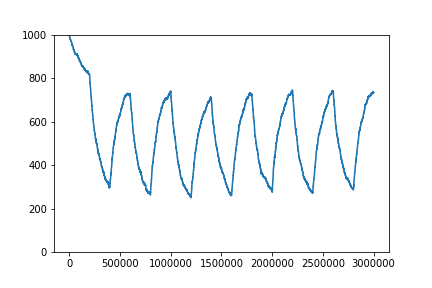
\includegraphics[width = 1.0\linewidth, trim={5 5 40 30}, clip=true]{figures/changing_selection_trajec.png}
		\subcaption{$n1$ as a function of simulated time}
		\label{fig:changing_constant_trajec}	
	\end{subfigure}
	\hspace{0.03\linewidth}
	\begin{subfigure}[t]{0.305\linewidth}
		\centering
		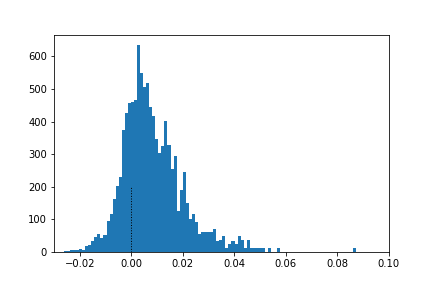
\includegraphics[width = 1.0\linewidth, trim={10 5 40 30}, clip=true]{figures/changing_selection_hist2.png}
		\caption{Frequency of fitnesses $f$ that fix in the population}
		\label{fig:changing_constant_hist}
	\hspace{0.03\linewidth}
	\end{subfigure}
	\begin{subfigure}[t]{0.305\linewidth}
		\centering
		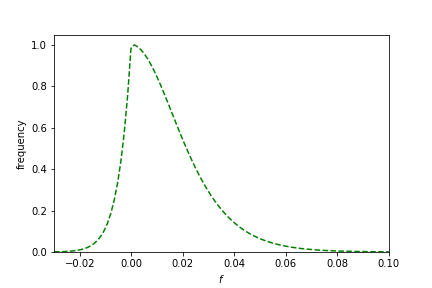
\includegraphics[width = 1.0\linewidth, trim={5 5 40 30}, clip=true]{figures/no_n_combined_dists.png}
		\caption{Predicted frequencies of fixation given by $e^{-\lambda |f|} p_{fix}(f)$}
		\label{fig:changing_constant_predict}
	\end{subfigure}
\caption{Simulated and predicted behavior of a system with constant $|f_i|$ and changing environment (scenario 2).}
\label{fig:changing_constant}
\end{figure}

In the long time limit of a changing environment, $\braket{n_1} = \braket{n_2}$ where $\braket{}$ denotes a time average. The frequency distribution is thus given by equations \ref{eq:dist1} and \ref{eq:dist2} with $n_1 = n_2 = 500$, giving
\begin{equation}\label{eq:shift_non}
y \propto exp(-|f|) * \dfrac{1- e^{-2 f}}{1- e^{-2 N f}}
\end{equation}
This has been plotted in figures \ref{fig:changing_resample_predict} and \ref{fig:changing_constant_predict} and we see that this theoretical distribution fits well with the data in both cases.

d)
As $\tau$ becomes large, changes in the environment become increasingly frequent, making the time average approximation increasingly accurate. This leads to the distribution of fitnesses that fix becoming increasingly similar to equation \ref{eq:shift_non} for both scenarios 1 and 2.

\begin{figure}[h]
	\centering
	\begin{subfigure}[t]{0.24\linewidth}
		\centering
		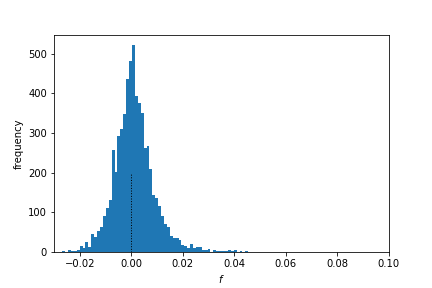
\includegraphics[width = 1.0\linewidth, trim={5 5 40 30}, clip=true]{figures/tau5e7_selection_hist2.png}
		\subcaption{$\tau = 10^{-7}$}
		\label{fig:t7}	
	\end{subfigure}
	\hspace{0.01\linewidth}
	\begin{subfigure}[t]{0.24\linewidth}
		\centering
		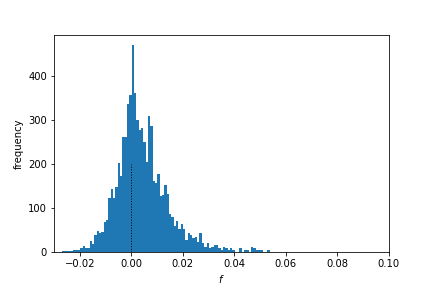
\includegraphics[width = 1.0\linewidth, trim={5 5 40 30}, clip=true]{figures/tau5e5_selection_hist2.png}
		\caption{$\tau = 10^{-6.5}$}
		\label{fig:t65}
	\end{subfigure}
	\begin{subfigure}[t]{0.24\linewidth}
		\centering
		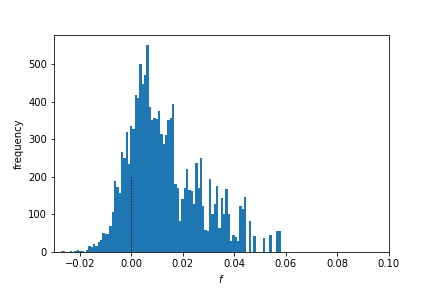
\includegraphics[width = 1.0\linewidth, trim={5 5 40 30}, clip=true]{figures/tau5e3_selection_hist2.png}
		\caption{$\tau = 10^{-4}$}
		\label{fig:t4}
	\end{subfigure}
	\begin{subfigure}[t]{0.24\linewidth}
		\centering
		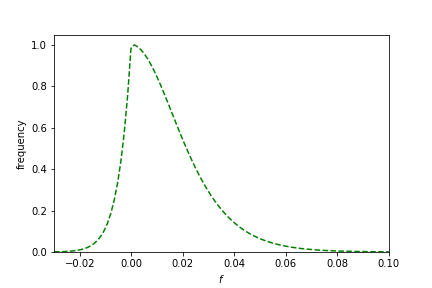
\includegraphics[width = 1.0\linewidth, trim={5 5 40 30}, clip=true]{figures/no_n_combined_dists.png}
		\caption{Predicted as $\tau, n \rightarrow \infty$}
		\label{fig:pred}
	\end{subfigure}
\caption{Frequency of fitnesses $f$ that fix in the population for a changing environment with fixed fitnesses $|f|$ (scenario 2). As $\tau$ increases, this increasingly resembles the predicted distribution resulting from a time average of the populations $n_1$ and $n_0$.}
\label{fig:changing_constant_taus}
\end{figure}

This can also be rationalized by looking at the $n_1$ curves where for small $\tau$ we only see a single or a few transitions, whereas for large $\tau$, transitions occur very rapidly and the equilibrium state has $n_1 \approx n_2 \approx 500$. Since the rapidly changing environment leads to $\braket{f_i^0} = \braket{f_i^1}$ over the timescale of mutagenesis, the frequency of fixation is simply proportional to the sampling frequency $exp(-|f|)$ times the probability of fixation$ \dfrac{1- e^{-2 f}}{1- e^{-2 N f}}$ in both states 0 and 1.

\begin{figure}[h]
	\centering
	\begin{subfigure}[t]{0.305\linewidth}
		\centering
		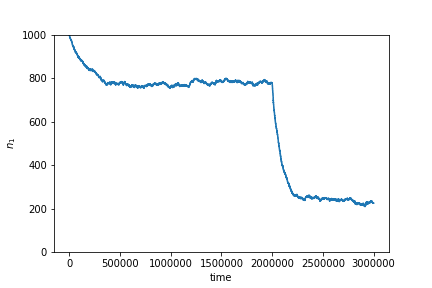
\includegraphics[width = 1.0\linewidth, trim={5 5 40 30}, clip=true]{figures/tau5e7_selection_trajec.png}
		\subcaption{$\tau = 10^{-7}$}
		\label{fig:t7}	
	\end{subfigure}
	\hspace{0.03\linewidth}
	\begin{subfigure}[t]{0.305\linewidth}
		\centering
		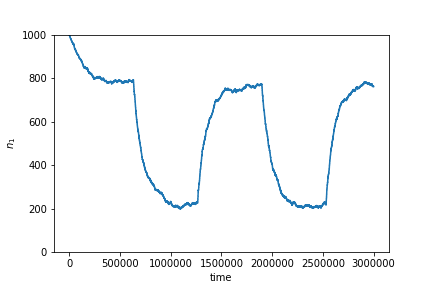
\includegraphics[width = 1.0\linewidth, trim={5 5 40 30}, clip=true]{figures/tau5e5_selection_trajec.png}
		\caption{$\tau = 10^{-6.5}$}
		\label{fig:t65}
	\end{subfigure}
	\hspace{0.03\linewidth}
	\begin{subfigure}[t]{0.305\linewidth}
		\centering
		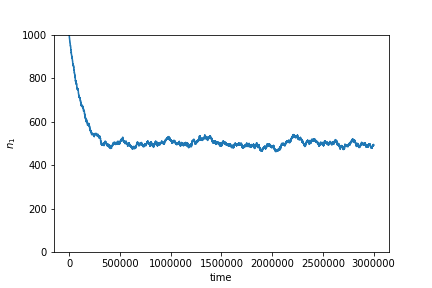
\includegraphics[width = 1.0\linewidth, trim={5 5 40 30}, clip=true]{figures/tau5e3_selection_trajec.png}
		\caption{$\tau = 10^{-4}$}
		\label{fig:t4}
	\end{subfigure}
\caption{$n_1$ as a function of simulated time for a changing environment with fixed $|f_i|$. As $\tau$ increases, oscillations become increasingly fast, allowing us to take a time average of the populations $n_1$ and $n_0$.}
\label{fig:changing_constant_trajecs}
\end{figure}

We thus see that as $\tau$ increases, the proportion of fixed mutations that are beneficial (i.e. has $f > 0$) increases until it reaches the limiting distribution given by equation \ref{eq:shift_non}.  In the case of constant fitnesses (scenario 2), a better fit to the predicted frequencies would be obtained with an increased number of genes.

\newpage

e)
\textit{Drosophila} have a relatively short generation time of $\approx$2 weeks. Changes in the environment due to factors such as changing seasons thus occur over a timescale that allows for fixation of mutations in small populations within a single season. This scenario is qualitatively similar to the scenario considered above, where e.g. alleles that are more beneficial during the summer can arise and fix during the warmer months while alleles that are more beneficial in the winter can arise and fix during the colder months. As exemplified by figures \ref{fig:changing_constant_taus} and \ref{fig:changing_constant_trajecs}, this will lead to the population having a large proportion of beneficial mutations if the relative timescales of the generation time (and thus time of fixation) and change in environment are appropriate.

As is evident from figure \ref{fig:changing_constant_trajecs}, this can lead to there being a number of beneficial mutations at any one time, but at a later time these may turn out to be detrimental and thus be cleared from the population. This does not lead to the mean fitness of the population increasing over long timescales, but it does lead to the population being fitter at a given time of year, although there will be a delay corresponding to the fixation time of the mutations.

This particular scenario is likely to be more similar to the model with resampling of fitnesses rather than fixed fitnesses since we can imagine there to be a set of mutations $\{1_j\}$ that are more beneficial during the summer and a set of mutations $\{0_j\}$ that are more beneficial during the winter, and while the population can change between these two states, it is unlikely that mutations are exactly reversed. Instead, the population will likely sample genotype space in a more continous manner where mutations in a given gene can have different fitness advantages depending on how they affect the resulting protein and its expression level.


{\textbf{notes to self}}

\begin{equation}
n1 \cdot p(a=1 \rightarrow a=0) = n2 \cdot  p(a=0 \rightarrow a=1)
\end{equation}

This implies that the integral of the right side of the above figure must be equal to the integral of the left side. We can thus calculate the expected n1 analytically.

\newpage






\subsection{Ancestral inference}
%What can we say about the time to the most recent common ancestor from which any pair of the MPhil students from the class of 2018-19 share inherited DNA?

a) %What theory would you use to estimate this time, and what parameters are required? Suggest some values for these parameters.}

We start by considering the genealogy at a single haploid locus ignoring recombination and mutation. An example of such a system might be human mtDNA.
A simple theory we can use to calculate the time to the most recent common ancestor (TMRCA) for a set of n individuals given a total population size of N in this scenario is the Kingman coalescent.
We start by assuming that reproduction follows a Wright-Fisher (WF) model and thus satisfies the following conditions:
\begin{enumerate}
\item Nonoverlapping generations
\item Random reproduction (Poission distributed offspring count)
\item Constant population size $N$
\item Random mating
\end{enumerate}

Now let $p(n)$ be the probability that none of $n$ individuals share a parent in the previous generation. We can use this to also calculate $1-p(n)$, the probability that a coalescence event does occur in the previous generation. Together, these two parameters allow us to calculate the distribution of $T(i)$ which we define as the time required for the first two of $i$ individuals to share a common ancestor. We assume that at most one coalescence event occurs per generation. Finding an expression for $T(i)$ also allows us to calculate the time to the most recent common ancestor $TMRCA$ of all $n$ individuals as
\begin{equation}
TMRCA = \sum_{i=2}^n{T(i)}
\end{equation}

Considering only $n=2$ individuals from a population of size $N$, the probability that they share an ancestor in the previous generation is $(1 - p(2)) = 1/N$ since mating is random in the WF model. This gives $p(2) = 1-1/N$. Consider now the case where $n=3$. In this case, we can calculate the probability of no shared ancestors as the probability of the first two individuals not having a shared ancestor ($1-1/N$) times the probability of the third individual not sharing ancestors with the first two ($1-2/N$):
\begin{equation}
p(3) = (1-1/N) * (1-2/N)
\end{equation}
Generalizing this to arbitrary n gives $p(n) = p(n-1) * (1-(n-1)/N)$. Using this inductive argument together with $p(2) = 1/N$, we get
\begin{equation}
p(n) = \prod_{i=1}^{n-1}{1-i/N} = 1 - \sum_{i=1}^{n-1}{\dfrac{i}{N}} + \mathcal{O}(1/N^2) = 1 - \dfrac{(n-1)n}{2N}+ \mathcal{O}(1/N^2)
\end{equation}

This is the probability that no individuals in a sample of $n$ share any ancestors in the previous generation given a population size of $N$.
Conversely we can also calculate the probability that at least two of the $n$ individuals share an ancestor in the previous generation which to first order is
\begin{equation}
1 - p(n) \approx \dfrac{n(n-1)}{2N}
\end{equation}

In the WF model, generations are independent such that the probability that $n$ individuals share no ancestors in $t$ generations is
$p(n| t) = p(n)^t$
Hence the probability that the first coaslescence event for the $n$ individuals occurs in generation t, $C(t|n)$, is the probability that no coalescence has occurred before then 
\begin{equation}
p(n)^{t} \approx (1 - \dfrac{n(n-1)}{2N})^t = 1 - \dfrac{n(n-1)}{2N} t + O(1/N^2) \approx e^{-\dfrac{n(n-1)}{2N} t}
\end{equation}
 times the probability that coalescence occurs in a given generation ($1-p(n) \approx \dfrac{n(n-1)}{2N}$). We can thus write this probability distribution as 
\begin{equation}\label{eq:coal}
C(t|n) = p(n)^{t} (1-p(n)) \approx  \dfrac{n(n-1)}{2N} e^{-\dfrac{n(n-1)}{2N} t}
\end{equation}
This is an exponential distribution with parameter $\lambda = \dfrac{n(n-1)}{2N}$,
\begin{equation}
p(t) = \lambda e^{-\lambda t}
\end{equation}
In the present case the above assumptions are justified since N is expected to be large, on the order of $10^3 - 10^4$, and $n$ is on the order of $10^1$.

This distribution has a mean of $E[T(i)] = 1 / \lambda =  \dfrac{2N}{i(i-1)}$ which is thus the expected time for two of the $i$ lineages to converge.
We note that the distribution also has a large variance of $Var[T(i)] = 1 / \lambda^2 =  (\dfrac{2N}{i(i-1)})^2$.

A reasonable question is now what value to choose for $N$. Here we could opt for the global mean effective population size of $N_e = 20,000$ quoted in the PG lecture notes. For the MPhil class with $n=19$ individuals, this corresponds to the first ancestor from which a single pair of MPhil students share inherited DNA at this locus having lived $T(19) = \dfrac{2*20000}{19(19-1)}=116.96$ generations ago with an identical standard deviation. The human generation time may be taken as approximately 25 years (Scally \& Durbin (2012) suggest a range of 20-30 years). This corresponds to the ancestor in question having lived 2429 years ago.

However, we could also consider the fact that the majority of the MPhil class (17 of 19) is of European ancestry where we can instead take $N_e \approx 1000$ (Melé et al. (2012)). Since $\lambda$ is linear in $N$, this corresponds to a common ancestor from which two individuals share DNA living only $T(17) = \dfrac{2*1000}{17(17-1)} * 25 = 163.4$ years ago.

If on the other hand we pick two students at random and ask when the most recent common ancestor from which they share DNA lived, the expected answer is $T(2) = N$ which is 1,000-20,000 generations depending on the effective population size we use for our calculation.

If instead we interpret the phrase "the most recent common ancestor from which any pair of the MPhil students share inherited DNA" to mean the most recent ancestor from which any pair of students we pick will have shared DNA at this locus, we need the TMRCA of the whole population. For a sample of $n$ individuals in a population of size $N$, this is
\begin{equation}
E[TMRCA] = \sum_{i=2}^n{E[T(i)]} = \sum_{i=2}^n{\dfrac{2N}{i(i-1)}} = 2N \sum_{i=2}^n{[\dfrac{1}{i-1}-\dfrac{1}{i}] = 2N(1-\dfrac{1}{n})}
\end{equation}
Given the size of the 2018/2019 MPhil class of 19 students with $N_e = 20000$, we thus get
\begin{equation}
E[TMRCA] = 2*20000(1 - 1/19) = 37,895 \text{ generations} = 947,368 \text{ years}
\end{equation}
This is of course an unreasonable estimate since this predates the out-of-Africa event by an order of magnitude. If instead we use $N_e = 1000$ we get $TMRCA = 47368$ years which seems more reasonable.

%We might also be interested in an expression for the variance of our estimate. Since our coalescence times are assumed to be independent, this is
%\begin{equation}
%Var[TMRCA] = \sum_{i=2}^n{Var[T(i)]} = \sum_{i=2}^n{[\dfrac{2N}{i(i-1)}]^2} = 4N^2 \sum_{i=2}^n{[\dfrac{1}{(i-1)^2}-\dfrac{2}{(i-1)}+\dfrac{1}{i^2}+\dfrac{2}{i}]} 
%\end{equation}
%\begin{equation}
%Var[TMRCA]  = 4N^2(\dfrac{2}{N}-2+1-\dfrac{1}{n^2}+2 \sum_{i=2}^{n-1}{\dfrac{1}{i^2}})
%\end{equation}
%As far as I am aware there is not a nice closed form solution for this sum, but we can easily calculate the result for $n=19$ in which case
%\begin{equation}
%Var[TMRCA]  = 4N^2(\dfrac{2}{19}-2+1-\dfrac{1}{19^2}+2 * 0.5909) = 1.137 N^2
%\end{equation}
%For the above case with $N_e = 1000$, the standard deviation is thus $\sigma = 26658$.

However, when considering the most recent common ancestor from which we share DNA, we need to consider not just haploid loci like the mitochondria but also take into account the fact that most of our DNA is diploid. In the Kingman coalescent, this is easily achieved by substituting $N \rightarrow 2N$ and then letting $n = 38$ since we are now considering both the maternal and paternall copy in each individuals such that there are 38 copies of each locus in the sample (Hudson 1990).

This gives a time to the most recent coalescence event of
\begin{equation}
E[T(i=38)] =  \dfrac{4N}{i(i-1)} = \dfrac{4*20,000}{38(38-1)} *25 =1422 \text{ years}
\end{equation}
For $N_e = 20,000$ and $E[T(i=38)] = 71 \text{ years}$ for $N_e = 1,000$. This first coalescence point will be the most recent common ancestor contributing DNA at this locus to two individuals with probability $p = 36/37$ while in the remaining $1/37$ cases, the first coalescence will be of two genes from the same individual (assuming random mating).

When considering the time of the most recent common ancestor from which the whole MPhil cohort share inherited DNA, we need to identify the first node in the coalescent that joins 19 individuals. This is unlikely to be the first node with 19 descendants since some of the coalesced haploid genomes can come from the same individual. Considering random sampling of the haploid genomes, the probability that all 19 individuals are represented by K genes sampled from a total of 38 with $K \in [19, 38]$ is given by
\begin{equation}
p_{all}(K) = \dfrac{N_{all}(K)}{\begin{pmatrix} 38 \\ K \end{pmatrix}} = \dfrac{2^{38-K} 19!}{(38-K)! (K-19)!} \dfrac{K! (38-K)!}{38!} = \dfrac{2^{38-K} K! 19!}{38!(K-19)!}
\end{equation}
Where $N_{all}(K)$ represents the number of ways to draw K samples from 38 haploid genomes such that all 19 individuals are represented. This distribution has been plotted in figure \ref{fig:sampKs}.

\begin{figure}[h]
	\centering
	\begin{subfigure}[t]{0.45\linewidth}
		\centering
		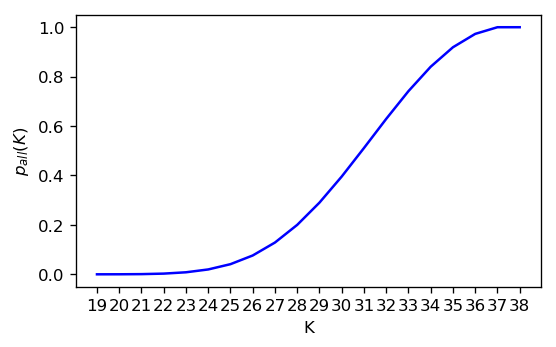
\includegraphics[width = 1.0\linewidth, trim={0 0 0 0}, clip=true]{figures/samp_K.png}
	\end{subfigure}
\caption{Probability that 19 indidividuals are represented when randomly sampling K genes from 38 haploid genomes.}
\label{fig:sampKs}
\end{figure}

We see that $p_{all}(K = 31) \approx 0.5$ and therefore for simplicity consider the most recent common ancestor of the full MPhil cohort to be the first ancestor of 31 leafnodes.
Of course the time of this node does not easily follow from the analytical treatment of the coalescent above but can be extracted from simulations as wil be discussed later.

For a real system, in addition to population size and generation time we also need to consider the fact that there is a finite recombination rate. This leads to separate sections of the genome having non-identical genealogies which must all be considered. In this case, the time to the most recent common ancestor from which DNA is shared for a pair of students is the most recent coalescence event in any tree. The time to the most recent common ancestor from which the full cohort shares DNA at a single locus is the time to the first node joining 31 leafnodes in any tree.

The coalescent with recombination is not easily treated analytically but we can simulate it using msprime (Kelleher et al. 2016) which will be discussed further in part (c). In msprime, we do not simulate the full Ancestral Recombination Graph (ARG) since most common ancestor events will be between lineages with no overlapping ancestral material. Instead, only events leading to coalescence at loci of interest are simulated and stored.

In addition to the number of samples, $n=38$, the population size $N_e$ and the generation time $T_{gen} \approx 25 \text{ years}$, we also need to estimate the recombination rate $\rho$ for these simulations. 
In this report, we will use a default recombination rate of $\rho = 0.5 \text{x} 10^{-9} \, \text{bp}^{-1} \text{year}^{-1} = 40 \, \text{generation}^{-1}$ as proposed by Scally and Durbin (2012).
\\


b) %What additional factors might modify this estimate? Estimate how they would affect it and by how much}.

Additional factors affecting the estimate are factors violating the Wright-Fisher assumptions.

One such factor is changing population size, and this is an important factor since we know that the global population has increased significantly over the past 100,000 years. As discussed above, the effective population size $N_e$ is usually used in population genetics rather than the actual population size. However, even the use of an appropriately time-averaged Ne for the process of interest  can be erroneous since the time-variation of $N_e$ can affect our coalescent both qualitatively and quantitatively.

The effects of varying $N_e$ can be quantified by considering Tajima's D.
Denoting the mutation rate by $\mu$, we can calculate the expected genetic difference rate between individuals as\\
$E(observed \,\, difference \,\, rate) = \theta_\pi = 2 N \mu$ \\
$\theta_\pi$ thus provides one measure of genetic diversity in terms of the pairwise genetic differences between individuals.

We can also quantify genetic diversity based on the number of segregating sites S.
\begin{equation}
E[S] = 2 \mu \sum_{i=2}^n{iT(i)}  = \theta \sum_{i=1}^{n-1}{\dfrac{1}{i}} \approx \theta \log{(n)}
\end{equation}
This allows us to define Watterson's theta as another measure of genetic diversity.
\begin{equation}
\hat \theta_S = \dfrac{S}{\sum_{i=1}^{n-1}{\dfrac{1}{i}}}
\end{equation}

Under the Wright-Fisher assumptions $\theta_\pi = \theta_S$, and Tajima's D for quantifying deviations from these assumptions is therefore defined as 
\begin{equation}
D = \dfrac{\hat \theta_\pi - \hat \theta_S}{\sqrt{(\hat \theta_\pi - \hat \theta_S)}}
\end{equation}
This is the scaled difference between the mean number of pairwise differences between individuals and the number of segregating sites. It is therefore sensitive to the number of rare mutations and thus to $N_e$.
If D is positive there is a deficiency of rare mutations in the current population, suggesting excess recent coalescences and thus a recent small Ne corresponding to a declining population

In this case, the most recent branches of the evolutionary tree would be shortened relative to the more distant branches which would be elongated. This might lead us to underestimate TMRCA if we base it on current population sizes and overestimate TMRCA if we base it on ancient population sizes. On the contrary if D is negative, there is an excess of rare mutations and recent branches of the coalescent will be longer than expected due to an increasing population size. In this case, we might overestimate TMRCA if we base it on current population sizes and underestimate TMRCA if we base it on ancient population sizes. These effects are illustrated in figure \ref{fig:changing_pop} for a set of simple simulations of haploid genomes.

\begin{figure}[h]
	\centering
	\begin{subfigure}[t]{0.305\linewidth}
		\centering
		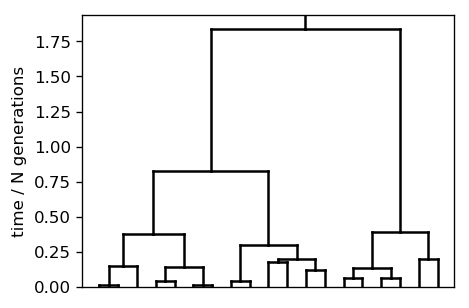
\includegraphics[width = 1.0\linewidth, trim={0 0 0 0}, clip=true]{figures/drawtree_constant.png}
		\subcaption{$D = 0$}
		%\label{fig:t7}	
	\end{subfigure}
	\hspace{0.03\linewidth}
	\begin{subfigure}[t]{0.305\linewidth}
		\centering
		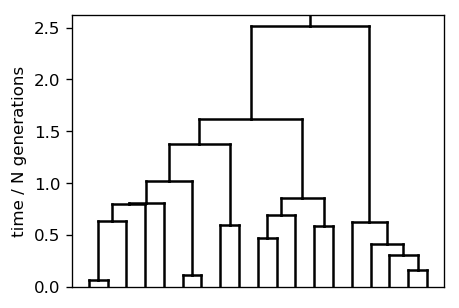
\includegraphics[width = 1.0\linewidth, trim={0 0 0 0}, clip=true]{figures/drawtree_increasing.png}
		\caption{$D < 0$}
		%\label{fig:t65}
	\end{subfigure}
	\hspace{0.03\linewidth}
	\begin{subfigure}[t]{0.305\linewidth}
		\centering
		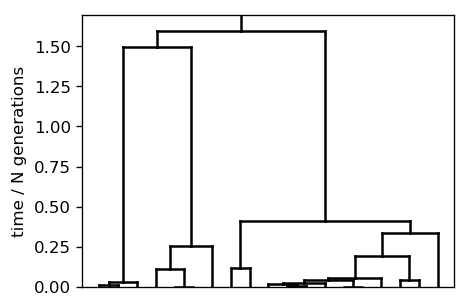
\includegraphics[width = 1.0\linewidth, trim={0 0 0 0}, clip=true]{figures/drawtree_decreasing.png}
		\caption{$ D > 0$}
		%\label{fig:t4}
	\end{subfigure}
\caption{Example trees for constant population size (D = 0), increasing population size (D $<$ 0) and decreasing population size (D $>$ 0) with $n=19$. Trees were simulated by drawing sequential coalescence events from the exponential distribution in equation \ref{eq:coal}.}
\label{fig:changing_pop}
\end{figure}

Since $E[TMRCA]$ is linear in $N$, the magnitude of the effects of changing population size could be rather large if we are considering long time periods over which the population size has changed significantly. However, if we use data for our effective population size that takes the changing population size into account, this should be mitigatable. This is hard to do in practice since our TMRCA events depend on Ne, but Ne depends on how much of human history we are considering.

Another violation of the Wright-Fisher model that may affect our estimate is population structure. The WF model assumes random mating in the population which is not true in structured populations. This approximation may be reasonable in isolated populations, but when considering larger populations it can make a significant difference. As already discusse in section (a), if we for example assume that all MPhil students are of European ancestry, this allows us to reduce the effective population size for the calculation by a factor of 10-20 compared to the case where we consider the global population, and this in turn affects the calculated TMRCA by an order of magnitude.

Additionally, if the cohort consists of people from different subpopulations, we might need further details in our model to take this into account. This is indeed the case in the present calculation since in the actual MPhil cohort, there are people of both Chinese and Indian descent, suggesting that we should consider the out-of-africa population more broadly rather than merely the European population. There are no MPhil students of recent African descent and we therefore do not have to consider the global effective population size.

Population structure affects not just the TMRCA estimate but also the form of the genealogy. In the present case where the majority of our sample is of European descent and a minority of Asian descent, we expect a smaller TMRCA for the Asian than European subpopulation, and a TMRCA of the full cohort that is bounded from below by the time of migration separating the two subpopulations. Further complications arise in the case of non-zero migration between such subpopulations as in e.g. the island hopping model also described by Hudson. The effects of separated populations and migration can be taken into account by simulating the system with variable and separate $N_e$ but this is hard to solve analytically. We therefore defer further discussions of this to section (c).

\textbf{c)}% Can you come up with an estimate and range?}

To come up with an estimate and range of the time to the most recent common ancestor from which the MPhil students share inherited DNA, we use the msprime software by Kelleher et al.

We start by considering the pair of MPhil students that share the most recent common ancestor from which they both inherit DNA at a locus. From a), we know that it is likely that the first coalescence event will have taken place between two of the 17 students with European ancestry rather than the two students with Asian ancestry.

A simple guess at the most recent common ancestor to two MPhil students might thus be obtained from a simple consideration of the number of ancestors of an individual which is $2^g$ going g generations back.
The total number of ancestors of the European part of the cohort is thus $17*2^g$ assuming no overlap between ancestors or generations. We can now consider the probability of a common ancestor as the probability of drawing two identical individuals when drawing $n = 17*2^g$ from a generation size of $N \approx 40$million, ignoring the probability that these are ancestors of the same individual. This probability is given by
\begin{equation}
P_{shared} = 1 - \dfrac{N!}{(N-n)!N^n}
\end{equation}
This probability is plotted as a function of the number of generations in figure \ref{fig:ngens}

\begin{figure}[h]
	\centering
	\begin{subfigure}[t]{0.45\linewidth}
		\centering
		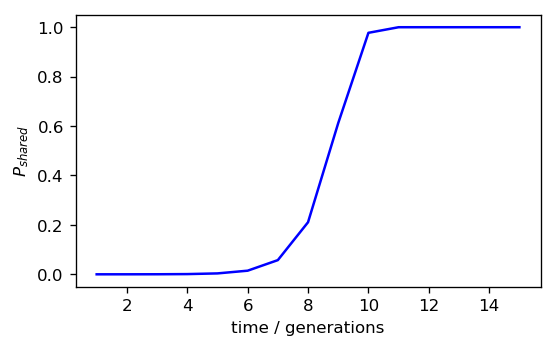
\includegraphics[width = 1.0\linewidth, trim={0 0 0 0}, clip=true]{figures/simple_ancestors.png}
	\end{subfigure}
\caption{Probability that $n = 17*2^g$ ancestors $g$ generations ago are not distinct.}
\label{fig:ngens}
\end{figure}

We thus see that there is a higher than 50\% probability that there is a shared ancestor 9 generations ago corresponding to 225 years ago, with a 90\% confidence interval of 175-250 years. This estimate might have to be modified slightly if the ancestors of the North-American part of the MPhil cohort emmigrated from Europe more than 250 years ago. However, with an increasing number of ancestors it becomes increasingly unlikely that a common ancestor event also represents a coalescence event.  In addition, it also becomes increasingly likely that the $2^g$ ancestors of a single individual are non-unique. Taken together, this suggests that our naive estimate might be an underestimate. We therefore return to the Kingman coalescent for an estimate that takes more details of the system into account.

The above considerations suggest that we are working with a relatively modern population, and it is thus unlikely to be appropriate with Ne=1000 as in section (a). Instead, we (somewhat arbitrarily) let Ne=100,000 (with Ne=1000, we get a most recent common ancestor living less than 1 generation ago).
Running 10 simulations, this gives a most recent common ancestor from which at least two MPhil students inherited DNA at the same locus having lived 335 years ago with a range of 190 to 541 years. If we were to also vary parameters such as effective population size and recombination rate, the variability in our estimate would be even greater.


%We also note that there are 34 separate haploid genomes in this sub-cohort corresponding to 544 unique pairs of haploid genomes from different individuals.
%As the expected first point of coalescence of any genomic region, we therefore take the first coalescence point at any site for a simulation with N=20,000, n=34, and $\rho = 0.5 \text{x} 10^{-9} \, \text{bp}^{-1} \text{year}^{-1}$ (Scally and Durbin) across the whole haploid genome.


To find the most recent common ancestor that has contributed DNA to the entire MPhil cohort assuming a homogenous population with random mating, we instead run a simulation with Ne=1,000. We simulate the full tree with n=38 leaves and for each locus  find the most recent common ancestor of all 19 individuals by finding the first node that is the ancestor of at least K leafnodes, with K drawn from equation \ref{eq:prob} for each site.

This gives a value of 473 generations corresponding to 11825 years since the most recent common ancestor to the entire cohort. When repeating this simulation 50 times, we get a mean of 13038 and standard deviation of 1136 for our estimate assuming a homogenous and randomly mating population. The resulting distribution is shown in figure \ref{fig:n1000_coals}
\begin{figure}[h]
	\centering
	\begin{subfigure}[t]{0.45\linewidth}
		\centering
		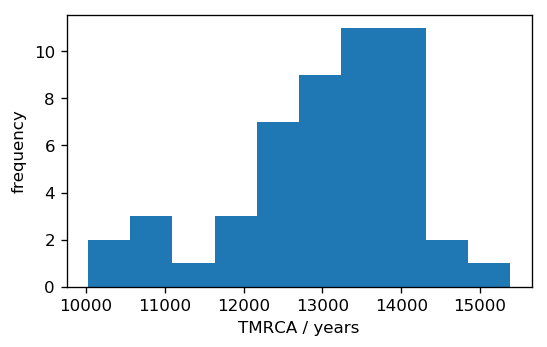
\includegraphics[width = 1.0\linewidth, trim={0 0 0 0}, clip=true]{figures/Ne1000_allcoal.png}
	\end{subfigure}
\caption{Distribution of TMRCA for 38 samples and Ne=1000.}
\label{fig:n1000_coals}
\end{figure}

However, to provide a range for our estimate we should include additional uncertainty in the parameters used and therefore repeat our simulation with $Ne \in [500, 3000]$, $t_{gen} \in [20, 30]$ and $\rho \in [0.25*10^{-9}, 1*10^{-9}]$. We run 100 simulations drawing all three parameters uniformly at random in the given ranges for each simulation and plot a histogram of the result in figure \ref{fig:randparams}
\begin{figure}[h]
	\centering
	\begin{subfigure}[t]{0.45\linewidth}
		\centering
		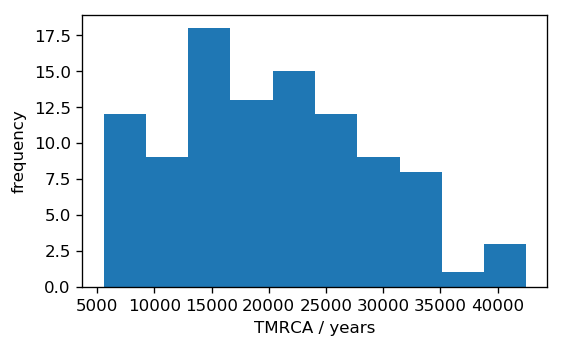
\includegraphics[width = 1.0\linewidth, trim={0 0 0 0}, clip=true]{figures/variableparams_allcoal2.png}
	\end{subfigure}
\caption{Distribution of time to the most recent ancestor from which all MPhil students share DNA at a single locus, drawing parameters uniformly at random as described in the main text.}
\label{fig:randparams}
\end{figure}

This gives us an expected value of 20,273 years, standard deviation of 8723 years and 90\% confidence interval of 7720 to 34993 years. We could also have considered the possibility that all pairs of MPhil students will share DNA from a single ancestor, but that different pairs of students share DNA at different loci. However, this is considered beyond the scope of the present assignment.

Finally we attempt to take into account population structure by considering Asian and European populations to have been completely separated since the European-Asian divergence 40,000-80,000 years ago (Scally \& Durbin).
It is clear from our previous simulations and calculations that at this point many loci in the current European MPhil cohort will have a single ancestor, and similarly the Asian MPhil cohort will likely have a single ancestor at many genetic loci.

The time to convergence for any single locus prior to the migration event will be on the order of $2N \approx 4000$ generations with an exponential distribution as discussed in (a). From our msprime simulations we expect on the order of  10,000 independently segregating loci with a single common ancestor 50,000 years ago. We therefore find the expected time to coalescence prior to migration as the $10^{-4}$ percentile of this exponential distribution, giving a value of $t_{coal} = - \text{ln}(\dfrac{1-1/10^{4}}{2(2-1)/4N}) = 0.2 \text{generations} = 5 years$. This suggests that the time to coalescence between the Asian and European MPhil lineages for the first locus to coalesce will be neglible after the migration event.

We verify this by running an msprime simulation with a migration event 50,000 years ago and find the TMRCA of the entire MPhil cohort at a single locus to have lived 2000.1 generations ago corresponding to 50,002.5 years.
A genealogy for an example locus from this simulation is given in figure \ref{fig:structure}

\begin{figure}[h]
	\centering
	\begin{subfigure}[t]{0.85\linewidth}
		\centering
		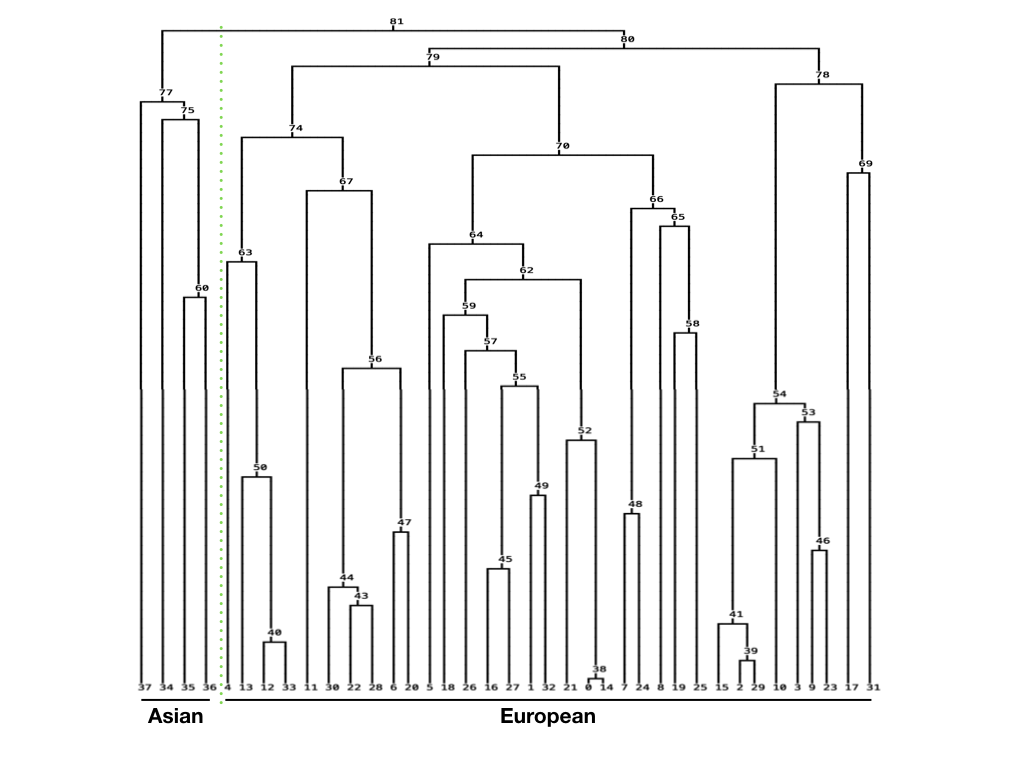
\includegraphics[width = 1.0\linewidth, trim={0 0 0 0}, clip=true]{figures/example_tree_msprime.png}
	\end{subfigure}
\caption{Example genealogy generated by msprime with a migration event 2000 generations ago separating the Asian samples (34, 35, 36, 37) from the European samples (0-33)}
\label{fig:structure}
\end{figure}

Hence in reality, the most recent ancestor contributing a section of DNA to the entire MPhil cohort is likely to have lived $\approx 50,000$ years ago with a range of 40,000-80,000 years as dictated entirely by the uncertainty in the European-Asian divergence. A low rate of migration between these populations since 50,000 years ago means that there is in practice a finite probability that the TMRCA is lower if this has caused mixing of the lineages.

In summary my best estimate at a most recent common ancestor that has contributed DNA to any two MPhil students lived 335 years ago with a range of 190 to 541 years while the most recent common ancestor that has contributed DNA to all MPhil students under the hypothesis of a homogenous population lived 20,273 years ago with a range of 7720 to 34,993 years. Taking into account the Asian-European divergence, my best estimate of the time to the most recent ancestor contributing a genomic segment to all MPhil students is 50,000 years with a range of 40,000 to 80,000 years corresponding to the time and uncertainty of the European-Asian divergence. If we pick a specific pair of students and want the TMRCA contributing shared genetic material to these two specific individuals, this is the expectation value of an msprime simulation with n=2 which yields 11378 years and a range of 2899 to 24680 years over 10 simulations if they are both of European descent, while we also expect a coalescence time of 40,000-80,000 years in this case if one is of European and one of Asian descent.


However, as the above analyses show, these estimates are strongly dependent on Ne, population structure, $\rho$ and the mean generation time. In particular, the effective population size and population structure of the relevant subpopulations have been very hard to estimate accurately, but while the estimates used in the present assignment may not be the most appropriate, they do at least illustrate how coalescent theory can be used to investigate common ancestor events for genetic loci in the absence and presence of recombination.

~\\

R. R. Hudson "Gene genealogies and the coalescent process" \textit{Oxford Surverys in Evolutionary Biology} (1991)\\
J. Kelleher et al. "Efficient Coalescent Simulation and Genealogical Analysis for Large Sample Sizes" \textit{PLOS Computational Biology} (2016)\\
M. Melé et al. "Recombination Gives a New Insight in the Effective Population Size and the History of the Old World Human Populations" \textit{Molecular Biology and Evolution} (2012)\\
A. Scally \& R. Durbin "Revising the human mutational rate: implications for understanding human evolution"  \textit{Nature Reviews Genetics} (2012)\\



\newpage

\subsection{Neanderthal introgression}

%Based on autosomal genome DNA analysis it is believed that Neanderthals hybridised with modern humans around the time they left Africa 60,000 years ago, resulting on a small frac- tion (1-2\%) of all non-African present day human autosomal genome sequence being derived from Neanderthals. However, in large numbers (say 1,000,000) of non-African mitochondrial genomes none of them match the Neanderthal mitochondrial genome.

a) %Assuming that there has been no selection, estimate the probability of seeing no Neanderthal mitochondria in modern people if there was 1\% contribution from Neanderthals to the out-of-Africa population 60,000 years ago. State what assumptions you have made in your model and what approximations if any in your calculation.

First we note a few key features of the problem at hand. Firstly, mitochondria are uniparentally, maternally inherited and we can thus consider the mitochondrial origin as a single trait analogous to the haploid single-locus case above. Secondly, we assume that there is no selective pressure such that mitochondria are randomly inherited. This means that if the population has a fraction $c$ of female individuals with Neanderthal mitochondria and $1-c$ female individuals with modern human mitochondria, there is a probability $c$  ($1-c$) that a given offspring receives Neanderthal (modern human) mitochondria. We also assume random mating, no population structure, non-overlapping generations and ignore mutations.

Following the argument of Nordborg (1998), when investigating a sample of $n$ modern humans we consider the distribution $g_{nk}(t=60,000 \text{years})$ that our $n$ current samples had $k$ ancestors $t$ years ago. For a given value of $k$, we can then calculate the probability that none of these ancestors had Neanderthal DNA as $p_k = (1-c)^k$ given the assumptions above. If none of the ancestors of our current samples had Neanderthal mitochondria, we will see no Neanderthal mitochondrial DNA in our $n=1,000,000$ modern humans and vice versa. Finally this allows us to calculate the probability that none of the $n$ modern humans have Neanderthal mitochondria as 
\begin{equation}\label{eq:prob}
P(0 | c, n, t) = \sum_{k=1}^{n}{g_{nk}(t)(1-c)^k}
\end{equation}

From Tavaré (1983) $g_{nk}(t)$ is given by
\begin{equation}\label{eq:gnk}
g_{nk}(t) = \sum_{i = k}^n{\rho_i^0(t) \dfrac{(2i-1)(-1)^{i-k} \, k_{(i-1)} \, n_{[i]}}{k! \, (i-k)! \, n_{(i)}}}
\end{equation}
Where $\rho_i^0(t) = \exp{(-i(i-1)t/(2N))}$ and we measure time in generations. $a_{(j)}$ and $a_{[j]}$ are defined as $a \, (a \pm 1) \, ... \, (a \pm (j-1) )$

To verify our implementation we first reproduce the results of Nordborg for a fixed population size with mixing times ($t_m$) of 100,000 and 30,000 years (figure \ref{fig:nordborg}). We see that in both cases the probability of observing no Neanderthal mitochondria in a modern sample of size $n=986$ with a female population size of $N = 3400$ and a generation time of 20 years decreases monotonously from 1 to 0 as c increases from 0 to 1.

\begin{figure}[h]
	\centering
	\begin{subfigure}[t]{0.45\linewidth}
		\centering
		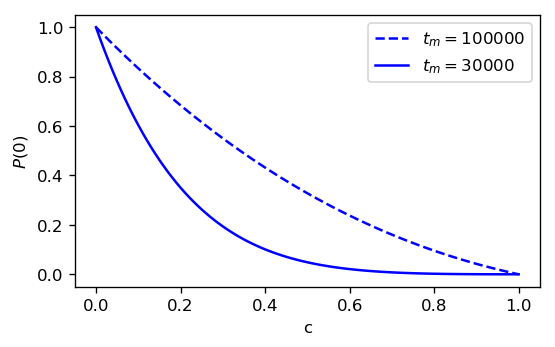
\includegraphics[width = 1.0\linewidth, trim={0 0 0 0}, clip=true]{figures/nordborg_curve.png}
	\end{subfigure}
\caption{Probability of oberserving no Neanderthal DNA in a modern sample of size $n=986$ as a function of c for two different mixing times (reproduced from Nordborg 1998).}
\label{fig:nordborg}
\end{figure}


We now return to the problem given in the assignment with $t=60,000$ years. We assume a generation time of 25 years as in question 3 and thus let $t = 2400$ generations.
Using equations \ref{eq:prob} and \ref{eq:gnk} with $c=0.01$, $n=1,000,000$ and $t=2,400$ with a population size of 20,000 and thus a female population size of N=10,000, we get $P(0|N=10,000) = 0.917$. This suggests a relatively small probability of observing Neanderthal DNA in modern humans under these hypotheses. Our calculation is thus consistent with a hypothesis of population mixing 60,000 years ago. If instead we let N=3400 as in Nordborg, we get $P(0|N=3400) = 0.968$, suggesting an even higher likelihood of not observing Neanderthal mitochondria in our modern sample.  To further investigate the relationship between N and $P(0|N)$, we plot $P(0)$ as a function of N in figure \ref{fig:Ncurve}.

\begin{figure}[h]
	\centering
	\begin{subfigure}[t]{0.45\linewidth}
		\centering
		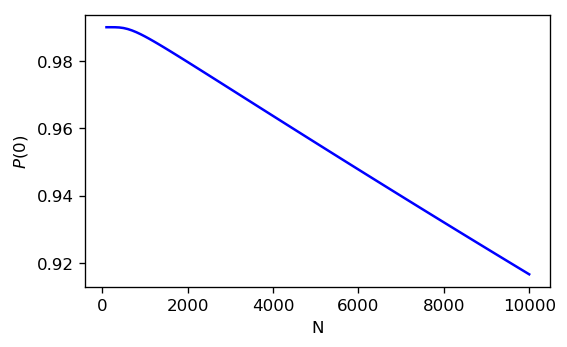
\includegraphics[width = 1.0\linewidth, trim={0 0 0 0}, clip=true]{figures/popN_curve.png}
	\end{subfigure}
\caption{Probability of oberserving no Neanderthal DNA in a modern sample of size $n=1,000,000$ as a function of female population size N over t=2400 generations.}
\label{fig:Ncurve}
\end{figure}

We see that after an initial plateau, $P(0)$ is approximately linearly decreasing in N. We can understand this intuitively since the expected number of ancestors of our sample increases with increasing N, and this in turn increases the probability that at least one of these had Neanderthal DNA, decreasing $P(0)$. The initial plateau at $P(0) = 0.99$ is the range of N for which we expect only a single ancestor of our sample.

However, we also note that all probabilities are relatively high. In light of section 1.3, this is understandable since we expect only a few ancestors 60,000 years ago even for N=10,000, and these are unlikely to have had any Neanderthal DNA with c=0.01. We therefore conclude that with $c=0.01$, the observation that none of our sample has Neanderthal mitochondria is a likely scenario.

b) %What is the equivalent probability if there was 10\% replacement? Discuss why this test has surprisingly little power even with large numbers of modern people.

If we let $c = 0.10$, the equivalent probabilities are $P(0|N=10000, c = 0.10) = 0.407$ and $P(0|N=3400, c = 0.10) = 0.718$. In this case, the term $(1-c)^k$  in equation \ref{eq:prob} becomes small much faster, resulting in a lower probability that no ancestors had Neanderthal mitochondria. To further investigate the effect of $c$ on $P(0)$, we follow the example of Nordborg and plot in figure \ref{fig:ccurve} $P(0)$ as a function of $c$ for both $N=10,000$ and $N=3400$.

\begin{figure}[h]
	\centering
	\begin{subfigure}[t]{0.45\linewidth}
		\centering
		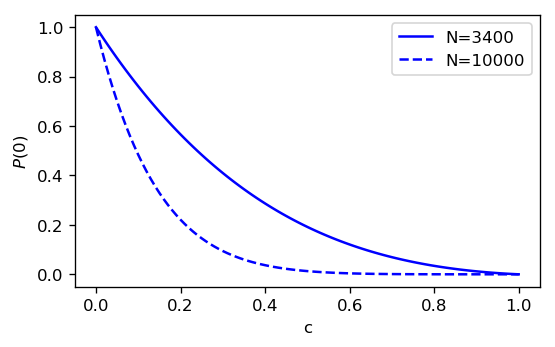
\includegraphics[width = 1.0\linewidth, trim={0 0 0 0}, clip=true]{figures/c_curve.png}
	\end{subfigure}
\caption{Probability of oberserving no Neanderthal DNA in a modern sample of size $n=1,000,000$ as a function of c after t=2400 generations.}
\label{fig:ccurve}
\end{figure}

As expected, we see that $P(0|N=10,000)$ very rapidly drops to 0 with c since with $N=10,000$ the expected number of ancestors 2,400 generations ago is $\braket{g_{10000, k}} = 8.67$ and $(1-c)^{8.67}$ rapidly goes to zero. In contrast $\braket{g_{3400, k}} = 3.19$ and the N=3400 curve therefore goes to zero more slowly. However, even with a population size of 10,000 and c=0.10, we cannot reject the hypothesis of population mixing 60,000 years ago on the basis of these simulations.

The reason why the calculated $P(0)$ values are quite high even with large numbers of modern people is that the entire population is likely to have only few ancient ancestors at the time of mixing as described above. This in turn results in $P(0)$ flattening as $n \rightarrow \infty$ as illustrated in figure \ref{fig:ncurve}.

\begin{figure}[h]
	\centering
	\begin{subfigure}[t]{0.45\linewidth}
		\centering
		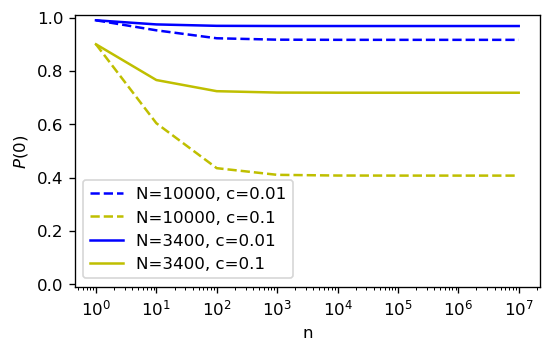
\includegraphics[width = 1.0\linewidth, trim={0 0 0 0}, clip=true]{figures/sampn_curve.png}
	\end{subfigure}
\caption{Probability of oberserving no Neanderthal DNA in a modern sample as a function of n with t=2400 generations and various N and c values.}
\label{fig:ncurve}
\end{figure}

The limiting value of $P(0|n)$ as $n \rightarrow \infty$ for a given $c, \, N$ is the probability that mitochrondrial DNA is completely lost from the population due to genetic drift (Tavaré 1983). We thus see that as soon as the sample size exceeds $\approx 1,000$ the probability that none of the sample contains Neanderthal mitochrondria is indistinguishable from the probability that the Neanderthal mitochrondria have been lost from the entire population, and increasing the modern sample size thus does not improve the statistical power of our analysis or our ability to determine whether a mixing event has taken place. We also note that in many of these cases our assumptions are obviously violated since we are sampling upwards of 1,000,000 individuals from a constant population of size 10,000, and this may affect our results at high n.

To investigate the time-dependency of the loss of Neanderthal mitochondria in the population, we can run an explicit simulation of the number of Neanderthal mitochondria present in each generation. We do this by drawing at each generation the number of female individuals with Neanderthal mitochondria ($n_i$) from a binomial distribution
\begin{equation}
n_{i+1} \sim \text{binomial}(Ne, n_i / Ne)
\end{equation}
We proceed to do this throughout the 2400 generations and plot the mean fraction of Neanderthal mitochondria over 10,000 simulations as a function of time in figure \ref{fig:simcourse}.

\begin{figure}[h]
	\centering
	\begin{subfigure}[t]{0.24\linewidth}
		\centering
		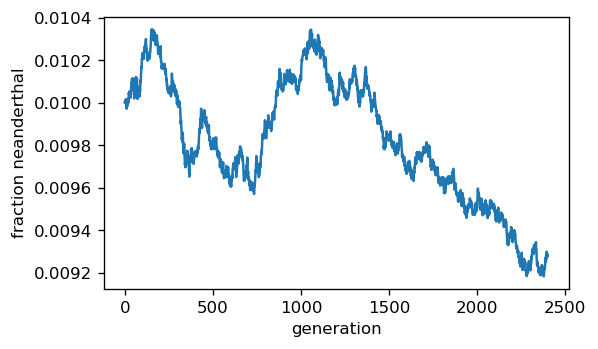
\includegraphics[width = 1.0\linewidth, trim={0 0 0 0}, clip=true]{figures/Ne3400_c01_meann.png}
		\subcaption{Ne=3400, c=0.01}
		%\label{fig:t7}	
	\end{subfigure}
	\hspace{0.0\linewidth}
	\begin{subfigure}[t]{0.24\linewidth}
		\centering
		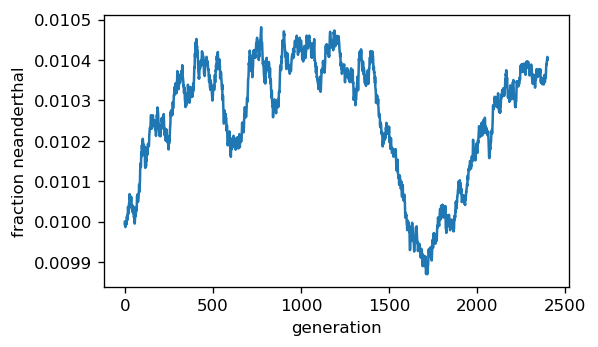
\includegraphics[width = 1.0\linewidth, trim={0 0 0 0}, clip=true]{figures/Ne10000_c01_meann.png}
		\caption{Ne=10,000, c=0.01}
		%\label{fig:t65}
	\end{subfigure}
	\hspace{0.0\linewidth}
	\begin{subfigure}[t]{0.24\linewidth}
		\centering
		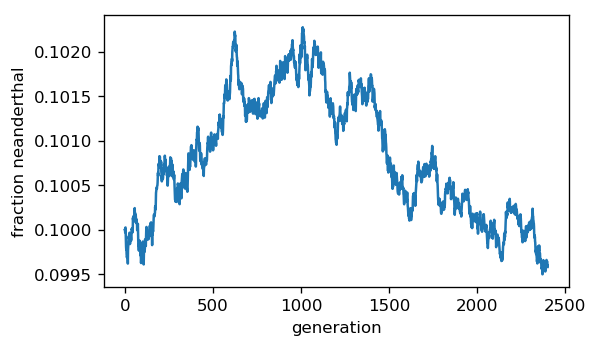
\includegraphics[width = 1.0\linewidth, trim={0 0 0 0}, clip=true]{figures/Ne3400_c1_meann.png}
		\caption{Ne=3400, c=0.10}
		%\label{fig:t4}
	\end{subfigure}
	\hspace{0.0\linewidth}
	\begin{subfigure}[t]{0.24\linewidth}
		\centering
		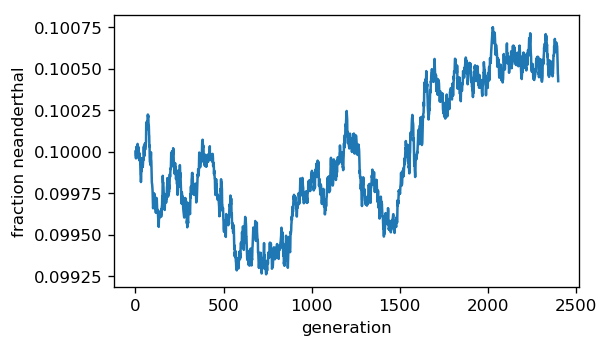
\includegraphics[width = 1.0\linewidth, trim={0 0 0 0}, clip=true]{figures/Ne10000_c1_meann.png}
		\caption{Ne=10,000, c=0.10}
		%\label{fig:t4}
	\end{subfigure}
\caption{Mean fraction of Neanderthal mitochondria over 10,000 simulations as a function of time since mixing.}
\label{fig:simcourse}
\end{figure}

Interestingly, we see that even though the proportion of Neanderthal mitochondria in any single simulation is very variable, the mean fraction of Neanderthal mitochrondria over 10,000 simulations remains approximately constant throughout the simulation. This is of course because $\braket{n_{i+1}} = n_i$ at every generation.

Consistent with the above considerations of allele loss, when looking at individual simulations we often observe complete loss of Neanderthal mitochrondria and thus fixation of modern human mitochondria. We show this in figure \ref{fig:histcourse} by plotting histograms of the time to loss of the last Neanderthal mitochrondrion.

\begin{figure}[h]
	\centering
	\begin{subfigure}[t]{0.24\linewidth}
		\centering
		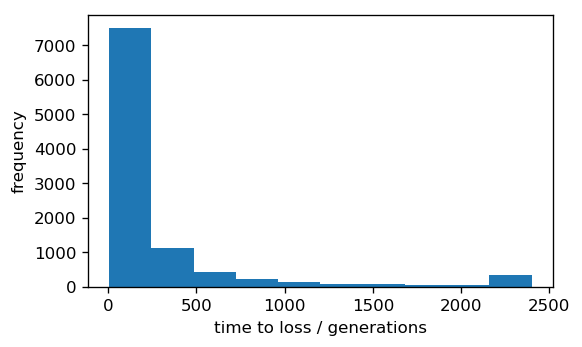
\includegraphics[width = 1.0\linewidth, trim={0 0 0 0}, clip=true]{figures/Ne3400_c01_histloss.png}
		\subcaption{Ne=3400, c=0.01\\P(0)=0.9698}
		%\label{fig:t7}	
	\end{subfigure}
	\hspace{0.0\linewidth}
	\begin{subfigure}[t]{0.24\linewidth}
		\centering
		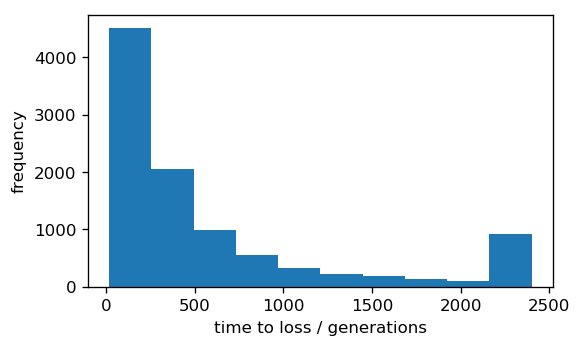
\includegraphics[width = 1.0\linewidth, trim={0 0 0 0}, clip=true]{figures/Ne10000_c01_histloss.png}
		\caption{Ne=10,000, c=0.01\\P(0)=0.9132 }
		%\label{fig:t65}
	\end{subfigure}
	\hspace{0.0\linewidth}
	\begin{subfigure}[t]{0.24\linewidth}
		\centering
		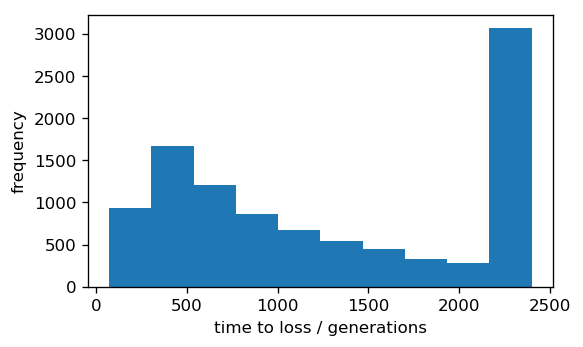
\includegraphics[width = 1.0\linewidth, trim={0 0 0 0}, clip=true]{figures/Ne3400_c1_histloss.png}
		\caption{Ne=3400, c=0.10\\P(0)=0.7186}
		%\label{fig:t4}
	\end{subfigure}
	\hspace{0.0\linewidth}
	\begin{subfigure}[t]{0.24\linewidth}
		\centering
		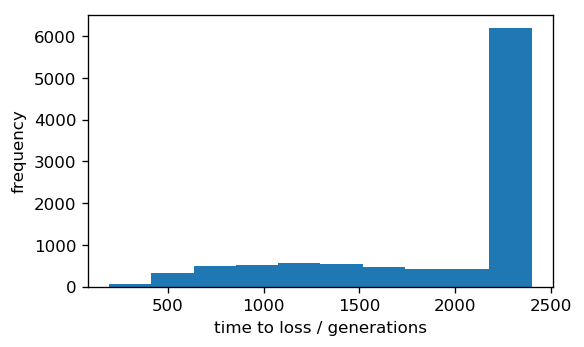
\includegraphics[width = 1.0\linewidth, trim={0 0 0 0}, clip=true]{figures/Ne10000_c1_histloss.png}
		\caption{Ne=10,000, c=0.10\\P(0)=0.4079}
		%\label{fig:t4}
	\end{subfigure}
\caption{Histogram of the time at which the last Neanderthal mitochondrion is lost from the population. Bars at 2400 represent the number of simulations where Neanderthal mitochondria are retained in the population. P(0) is 1 minus this fraction and is given under each histogram.}
\label{fig:histcourse}
\end{figure}

Finally we also plot in figure \ref{fig:histend} histograms of the proportion of Neanderthal mitochondria at the end of each simulation. We see that in the simulations where these are retained, they have often achieved relatively high frequencies which prevents loss by genetic drift. However, fixation of Neanderthal mitochrondria is rare with any of the parameter sets used.

\begin{figure}[h]
	\centering
	\begin{subfigure}[t]{0.24\linewidth}
		\centering
		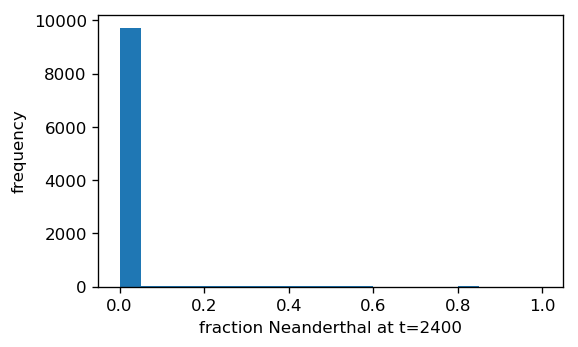
\includegraphics[width = 1.0\linewidth, trim={0 0 0 0}, clip=true]{figures/Ne3400_c01_histfrac.png}
		\subcaption{Ne=3400, c=0.01}
		%\label{fig:t7}	
	\end{subfigure}
	\hspace{0.0\linewidth}
	\begin{subfigure}[t]{0.24\linewidth}
		\centering
		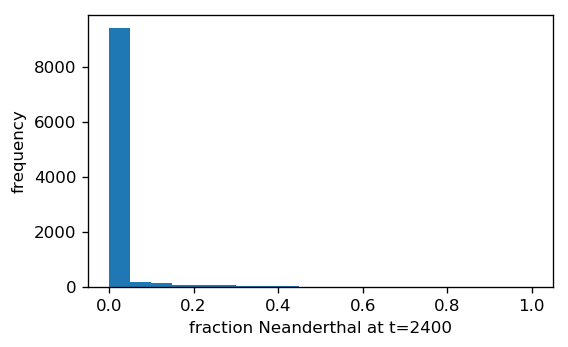
\includegraphics[width = 1.0\linewidth, trim={0 0 0 0}, clip=true]{figures/Ne10000_c01_histfrac.png}
		\caption{Ne=10,000, c=0.01}
		%\label{fig:t65}
	\end{subfigure}
	\hspace{0.0\linewidth}
	\begin{subfigure}[t]{0.24\linewidth}
		\centering
		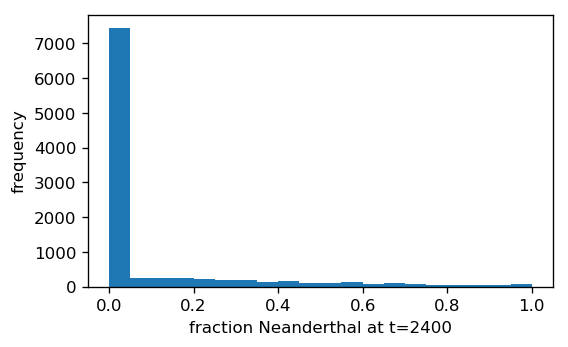
\includegraphics[width = 1.0\linewidth, trim={0 0 0 0}, clip=true]{figures/Ne3400_c1_histfrac.png}
		\caption{Ne=3400, c=0.10}
		%\label{fig:t4}
	\end{subfigure}
	\hspace{0.0\linewidth}
	\begin{subfigure}[t]{0.24\linewidth}
		\centering
		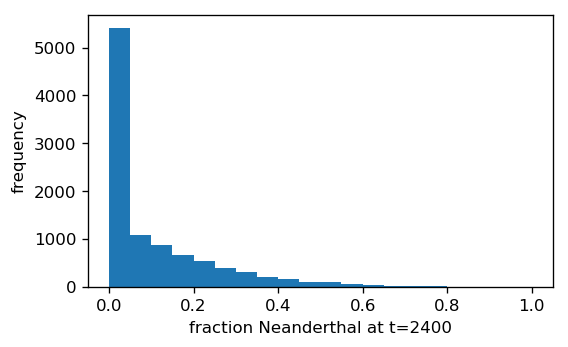
\includegraphics[width = 1.0\linewidth, trim={0 0 0 0}, clip=true]{figures/Ne10000_c1_histfrac.png}
		\caption{Ne=10,000, c=0.10}
		%\label{fig:t4}
	\end{subfigure}
\caption{Histograms of the fraction of Neanderthal mitochondria at the end of the simulation.}
\label{fig:histend}
\end{figure}

From figure \ref{fig:histcourse} we also see that the proportion of simulations where Neanderthal mitochondria are lost are very similar to what we arrived at using the approach of Nordborg. Given our large sample size of $n=10^6$ and finite $c(t = 2400)$ (figure \ref{fig:histend}), we can ignore the neglible probability that Neanderthal mitochrondria are retained in the population but not present in the sample as also discussed above. A direct comparison is given in table \ref{tab:comparison} where we see that the results from the simulation and equation \ref{eq:prob} agree to two decimal places. This suggests that we can use such simulations with high accuracy to model more complex scenarios that are not easily treated analytically.

\begin{table}[h]
\centering
\begin{tabular}{ |c c c c|}
\hline
 Ne & c & calculated P(0) (Nordborg) & simulated P(0) \\
\hline
3400 & 0.01 & 0.968 & 0.970 \\
%\hline
10,000 & 0.01 & 0.917 & 0.916 \\
%\hline
3400 & 0.10 & 0.718 & 0.719 \\
%\hline
10,000 & 0.10 & 0.407 & 0.408 \\
%\hline
\hline
\end{tabular}
\caption{Predicted P(0) using Nordborg's calculation and our simple simulation.}
\label{tab:comparison}
\end{table}

Given the consistency of table \ref{tab:comparison}, we can use similar simulations to easily investigate the effect of changing population size on P(0). In this case, we again use similar parameters to Nordborg, letting Ne increase from $3400$ to $10^9$ over 2000 generations starting 50,000 years ago according to $Ne = \text{max}(3400, 3400 \, \exp{(0.00630*(t-399))}$. The resulting probabilities are given in table \ref{tab:expsim} for c=0.01 and c=0.10 together with the corresponding probabilities for constant population sizes.

\begin{table}[h]
\centering
\begin{tabular}{ |c c c |}
\hline
 Ne & c & simulated P(0) \\
\hline
3400 & 0.01 & 0.970 \\
%\hline
10,000 & 0.01 & 0.916 \\
%\hline
exponential & 0.01 &  0.876   \\
%\hline
3400 & 0.10 &  0.719 \\
%\hline
10,000 & 0.10 & 0.408 \\
%\hline
exponential & 0.10 &  0.278 \\
%\hline
\hline
\end{tabular}
\caption{Predicted P(0) for constant and exponentially growing population sizes.}
\label{tab:expsim}
\end{table}

We thus see that with the more realistic increasing population size, it becomes significantly less likely that all Neanderthal mitchondria are lost from the population. However, P(0) is still greater than 0.25 for c=0.10 suggesting that even with this higher mixing ratio we still cannot with high probability discard the hypothesis that \textit{Homo sapiens} and Neanderthals mixed 60,000 years ago followed by loss of Neanderthal mitochrondria.

Finally we plot P(0) as a function of c for the exponentially increasing population, running 10,000 simulations for each value of c (figure \ref{fig:exp_ccurve}).

\begin{figure}[h]
	\centering
	\begin{subfigure}[t]{0.45\linewidth}
		\centering
		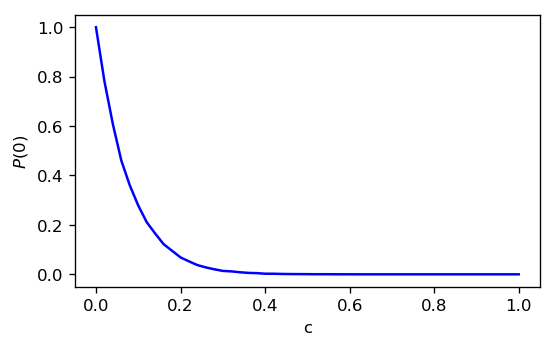
\includegraphics[width = 1.0\linewidth, trim={0 0 0 0}, clip=true]{figures/ccurve_exp.png}
	\end{subfigure}
\caption{Probability of oberserving no Neanderthal DNA in a modern sample as a function of c with exponential popoulation growth as described in the main text.}
\label{fig:exp_ccurve}
\end{figure}

We see that while there is a substantial probability of loss for $c < 0.20$, this probability decreases to  $P(0) < 0.01$ for $c > 0.33$. On the basis of our simulations, we thus conclude that there is unlikely to have occurred a mixing event between Neanderthals and modern humans with a mixing ratio of Neanderthals higher than 20\%, but a mixing ratio of 1-2\% as suggested by autosomal DNA analyses is very plausible.

c) %What biological factors might be important in determining the actual likelihood of observing Neanderthal mitochondria in modern humans which were not included in your model, and qualitatively what effect they would have.

Other biological factors influencing the estimate include selection, mating bias and population structure.

One might expect that if the majority of the population after mixing consisted of \textit{Homo sapiens} and the majority of nuclear DNA therefore had modern human origins, there would be a selective pressure against Neanderthal mitochondria. This is the case since a number of metabolic processes depend on coordination between nuclear and mitochondrial proteins, and the expression levels of these must therefore be appropriately balanced. This selective pressure would lead to a higher probability of lines with Neanderthal mitochondrial ancestry dying out, and would therefore increase P(0), the probability of not observing any Neanderthal mitochondria in the modern sample. In the simulated model, this selective pressure could for example be included by using an augmented c that is not merely the proportion of the population with Neanderthal mitochondria but also takes into account the probability that an individual with Neanderthal mitochondria will achieve reproductive success.

In the model, we have also assumed random mating which may not be the case. We might expect biased mating of Neanderthals with Neanderthals and \textit{Homo sapiens} with \textit{Homo sapiens}. In this case, the full population could be modelled as two sub-populations with migration, and if modern humans are descended from the \textit{Homo sapiens} sub-population, this would again decrease the probability of observing Neanderthal mitochondria in the modern sample and thus increase P(0) since the effective c would be smaller than the full Neanderthal mixing ratio.

This already touches upon the topic of population structure where we have assumed a single homogenous population in the above which may not be the case. The presence of subpopulations would for example increase the probability of loss of Neanderthal mitochondria by reducing the effective population size even if there is random mating within the subpopulations. From Nordborg and the considerations in section 1.3 and part (b), we also know changing population size to be important for the coalescent and the probability of allele loss. In the final section of part (b), we have attempted to take into account the growing global population instead of using an average effective population size, but this could also be modelled in more detail. . 

In summary, the proposed scenario of population mixing 60,000 years ago appears to be consistent with the observation that no modern humans contain Neanderthal mitochondria based on calculations and simulations with a range of population sizes and mixing ratios.
In contrast, Neanderthal DNA is still found in the nuclear genome where the coalescence timescale is slower, loss from genetic drift is slower, and recombination allows for decoupling of different loci.

~\\

M. Nordborg "On  the Probability of Neanderthal Ancestry" \textit{American Journal of Human Genetics} (1998)\\
S. Tavaré "Line-of-Descent and Genealogical Processes and Their Application in Population Genetics Models" \textit{Theoretical Population Biology} (1984)\\

\newpage

\section*{Appendix}

\lstinputlisting[language=python]{trees.py}

\lstinputlisting[language=python]{selection.py}

\lstinputlisting[language=python]{ancestral.py}

\end{document}

Estimate Ne from literature and give range pm standard deviation


We can also investigate these results by simulation. We simulate the coalescent as follows:
\begin{enumerate}

\item draw coalescence time from $p( t) = \dfrac{n(n-1)}{2N} e^{- \dfrac{n(n-1)}{2N} t}$

\item randomly join two lines

\item decrement n

\item repeat until n=1
\end{enumerate}

For the purpose of this simulation we scale by the population size N and let n=19. Three example coalescents are given in figure xxx

\begin{figure}[h]
	\centering
	\begin{subfigure}[t]{0.44\linewidth}
		\centering
		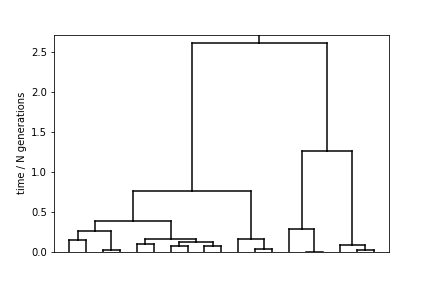
\includegraphics[width = 1.0\linewidth, trim={0 0 0 0}, clip=true]{figures/simtree1.png}
		\subcaption{}
		\label{fig:}	
	\end{subfigure}
	\hspace{0.01\linewidth}
	\begin{subfigure}[t]{0.44\linewidth}
		\centering
		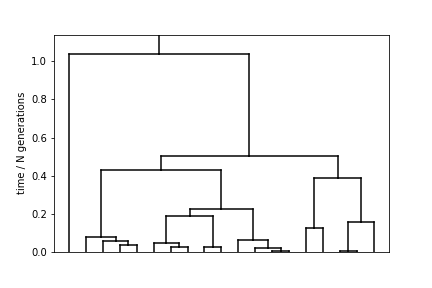
\includegraphics[width = 1.0\linewidth, trim={0 0 0 0}, clip=true]{figures/simtree2.png}
		\caption{}
		\label{fig:}
	\end{subfigure}
\caption{}
\label{}
\end{figure}

\begin{figure}[h]
	\centering
	\begin{subfigure}[t]{0.44\linewidth}
		\centering
		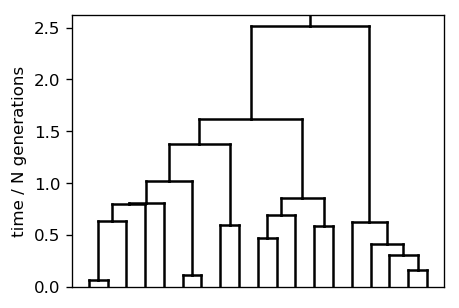
\includegraphics[width = 1.0\linewidth, trim={0 0 0 0}, clip=true]{figures/drawtree_increasing.png}
		\subcaption{}
		\label{fig:}	
	\end{subfigure}
	\hspace{0.01\linewidth}
	\begin{subfigure}[t]{0.44\linewidth}
		\centering
		\includegraphics[width = 1.0\linewidth, trim={0 0 0 0}, clip=true]{figures/drawtree_decreasing.png}
		\caption{}
		\label{fig:}
	\end{subfigure}
\caption{}
\label{}
\end{figure}


\begin{figure}[h]
	\centering
	\begin{subfigure}[t]{0.44\linewidth}
		\centering
		\includegraphics[width = 1.0\linewidth, trim={0 0 0 0}, clip=true]{figures/changing_N.png}
		\subcaption{}
		\label{fig:}	
	\end{subfigure}
\caption{}
\label{}
\end{figure}

We can also simulate 100 coalescents and plot the distribution of TMRCAs. This has mean xxx and standard deviation yyy as expected from our analytical considerations. Finally we try letting Ne vary over the course of the simulation, and we try including subpopulations. Consult literature!

we get:
mean: 1.898043429701977 var: 1.1725792272909699

\begin{figure}[h]
	\centering
	\begin{subfigure}[t]{0.44\linewidth}
		\centering
		\includegraphics[width = 1.0\linewidth, trim={0 0 0 0}, clip=true]{figures/tmrca_hist.png}
		\subcaption{}
		\label{fig:}	
	\end{subfigure}

\caption{}
\label{}
\end{figure}

We could add mutations to this simulation by first generating the coalescent, then sampling mutations on the tree.


	
Humans are diploid, so $\theta_\pi = 4Ne \mu$, where Ne is the effective population size. This gives $Ne = \dfrac{\theta_\pi}{4 \mu}$
For humans, $\theta_\pi \approx 0.001$, but $\mu$ is hard to estimate independently of $N_e$.




Cannot count all humans; european and american ancestry. Also not total population size. European population in 1600?
Although of course Aaditya is from India and Ronald is of Chinese descent which complicates things.
What's effective population size???

From the lectures:

Can add mutation by first constructing the coalescent, then sampling mutations on the tree. S is number of mutations (segregating sites). Setting N=1, 



\begin{enumerate}
\item changing population size

\item population structure
\end{enumerate}



Population outgrowth: long tips!. Population ingrowth: long stems!

Can quantify change in population size using Tajima's D




Tenesa et al.: bottleneck 20000 years ago; Ne is is 3100 for china and central europe. How to combine?
Mele lower  - myabe 800. Our estimate is linear in N so clearly lots of noise...


a) Assuming that there has been no selection, estimate the probability of seeing no Ne- anderthal mitochondria in modern people if there was 1\% contribution from Neanderthals to the out-of-Africa population 60,000 years ago. State what assumptions you have made in your model and what approximations if any in your calculation.

We assume that 60,000 years ago, 1\% of mitochondrial DNA was from Neanderthals (but no recombination in mitochondria no? maternal inheritance? is all or nothing?)

We assume that 60,000 years ago, 1\% of people had Neanderthal mitochondria. We assume that mitochondria are maternally inherited such that any offspring receive 100\% of their mitochondria from their mother. We assume that there is no fitness difference between Neanderthal and non-Neanderthal mitochondria. We assume a generation time of 25 years and the 60,000 years thus correspond to 2400 generations.

Assuming a constant population size of N, the number of Neanderthal mitochondria in generation 2 is given by a binomial distribution
\begin{equation}
p_1(n) = 0.99^n 0.01^{N-n} * \dfrac{N!}{n!(N-n)!}
\end{equation}

After 2400 generations, the probability is a product of 2400 such distributions.

I.e.
\begin{equation}
p_2(n) = \dfrac{N!}{n!(N-n)!} \int_0^\infty{p(n') (\dfrac{n'}{N})^n (\dfrac{N-n'}{N})^{N-n} dn'}
\end{equation}
This is not nice...

b) What is the equivalent probability if there was 10\% replacement? Discuss why this test has surprisingly little power even with large numbers of modern people.

c) What biological factors might be important in determining the actual likelihood of observing Neanderthal mitochondria in modern humans which were not included in your model, and qualitatively what effect they would have.


